\documentclass[10pt,a4paper]{scrartcl}
\usepackage{graphicx}



\usepackage[
    pdftitle={Abschlussarbeit},
    pdfsubject={Abschlussarbeit},
    pdfauthor={Aland Mariwan}
    pdfkeywords={Abschlussarbeit},
    pdftex=true,
    breaklinks=true,
    colorlinks=blue,
    citecolor=black,
    linkcolor=black,
    menucolor=black,
    urlcolor=black,
    colorlinks=true,
    filecolor=magenta,
    pdfpagemode=FullScreen,
 ]{hyperref}


 \usepackage[scaled]{uarial}
 \renewcommand*\familydefault{\sfdefault}
 \usepackage[T1]{fontenc}

% Standard Packages
\usepackage[utf8]{inputenc}
\usepackage[ngerman]{babel}
\usepackage[T1]{fontenc}
\usepackage{lmodern}
\usepackage{acronym}
\usepackage{amsmath}
\usepackage{longtable}
\usepackage{multirow}
\usepackage{tabulary}
\usepackage{booktabs}
\usepackage{caption}
\usepackage{siunitx}% align numbers at the decimal point
\usepackage{graphicx, subfig}
\graphicspath{{png/}}
\graphicspath{{jpg/}}
\graphicspath{{jpeg/}}
\usepackage{hyperref}
\usepackage{calc}
\usepackage{pdfpages}
\usepackage{xcolor}
\usepackage{booktabs}
\usepackage{tabularx}
\usepackage{enumitem}

\setlist{nolistsep}

\definecolor{blue}{HTML}{008ED7}
\definecolor{darkblue}{HTML}{00004e}
\definecolor{mygray}{gray}{0.75}
\definecolor{lightBlue}{HTML}{e5f7ff}
\definecolor{babyblue}{rgb}{0.54, 0.81, 0.94}
\definecolor{Gray}{gray}{0.9}

\renewcommand{\familydefault}{\sfdefault}
\renewcommand{\arraystretch}{1.5}

\usepackage{fancyhdr}
\usepackage{helvet}% text font
\renewcommand{\familydefault}{\sfdefault}
\pagenumbering{arabic}
\setcounter{page}{1}
\usepackage{color, colortbl}


% zusätzliche Schriftzeichen der American Mathematical Society
\usepackage{amsfonts}
\usepackage{amsmath}
\usepackage{color}
\usepackage{listings}
\renewcommand{\lstlistlistingname}{Quellcodesverzeichnis}

\usepackage{tgtermes}
\usepackage[left=2cm,right=3cm]{geometry}
\usepackage{setspace}
\usepackage[utf8]{inputenc}
% default encoding *last*
\usepackage[T2A,T1]{fontenc}
\usepackage[backend=biber,style=numeric]{biblatex}
\usepackage{csquotes}
\renewcommand\lstlistingname{Quellcode} %

%nicht einrücken nach Absatz
\setlength{\parindent}{0pt}
\usepackage[titletoc,toc,title,page]{appendix}

\setstretch{1.0}


% ============= Kopf- und Fußzeile =============
\usepackage{fancyhdr}
\pagestyle{fancy}
\fancyhf{}
\addtolength{\headheight}{1.5cm} % make more space for the header
%
\fancyhead[L]{\fontsize{8}{9}\bfseries Entwicklung einer Überwachung für Anwendungen\par}
\fancyhead[R]{
\includegraphics[width=60mm,height=10mm]{img/gssd.png}}
%%
\pagestyle{fancy}
\fancyfoot[L]{Aland Mariwan}
\fancyfoot[R]{\footnotesize Seite \thepage}
\renewcommand{\headrulewidth}{0.4pt}
\renewcommand{\footrulewidth}{0pt}
\newcommand{\ibx}[1]{\textbf{\textit{#1}}}
\newcommand{\iby}[1]{\textit{\textbf{#1}}}
\newcommand{\ibz}[1]{\textit{\bfseries #1}}


% Requires package: color.
\definecolor{mediumgray}{rgb}{0.3, 0.4, 0.4}
\definecolor{mediumblue}{rgb}{0.0, 0.0, 0.8}
\definecolor{forestgreen}{rgb}{0.13, 0.55, 0.13}
\definecolor{darkviolet}{rgb}{0.58, 0.0, 0.83}
\definecolor{royalblue}{rgb}{0.25, 0.41, 0.88}
\definecolor{crimson}{rgb}{0.86, 0.8, 0.24}

\lstdefinelanguage{JavaScript}{
  morekeywords=[1]{break, continue, delete, else, for, function, if, in,
    new, return, this, typeof, var, void, while, with},
  % Literals, primitive types, and reference types.
  morekeywords=[2]{false, null, true, boolean, number, undefined,
    Array, Boolean, Date, Math, Number, String, Object},
  % Built-ins.
  morekeywords=[3]{eval, parseInt, parseFloat, escape, unescape},
  sensitive,
  morecomment=[s]{/*}{*/},
  morecomment=[l]//,
  morecomment=[s]{/**}{*/}, % JavaDoc style comments
  morestring=[b]',
  morestring=[b]"
}[keywords, comments, strings]


\definecolor{chatgpt_light_gray}{RGB}{237, 237, 237}
\definecolor{chatgpt_light_blue}{RGB}{49, 130, 206}
\definecolor{chatgpt_light_green}{RGB}{56, 173, 169}
\definecolor{chatgpt_light_purple}{RGB}{163, 78, 194}

\lstdefinestyle{js}{
  language=JavaScript,
  basicstyle=\ttfamily\footnotesize,
  commentstyle=\color{chatgpt_light_green},
  identifierstyle=\color{black},
  numberstyle=\color{black},
  numbers=left,
  stepnumber=1,
  numbersep=5pt,
  breakatwhitespace=false,
  breaklines=true,
  captionpos=b,
  keepspaces=true,
  showspaces=false,
  showstringspaces=false,
  showtabs=false,
  tabsize=5,
  columns=flexible,
  frame=none,
  framexleftmargin=0pt,
  xleftmargin=10pt,
  framexrightmargin=0pt,
  framextopmargin=0pt,
  framexbottommargin=0pt
}


% ============= Package Einstellungen & Sonstiges =============
%Besondere Trennungen
\hyphenation{De-zi-mal-tren-nung}
% ============= Dokumentbeginn =============
\begin{document}
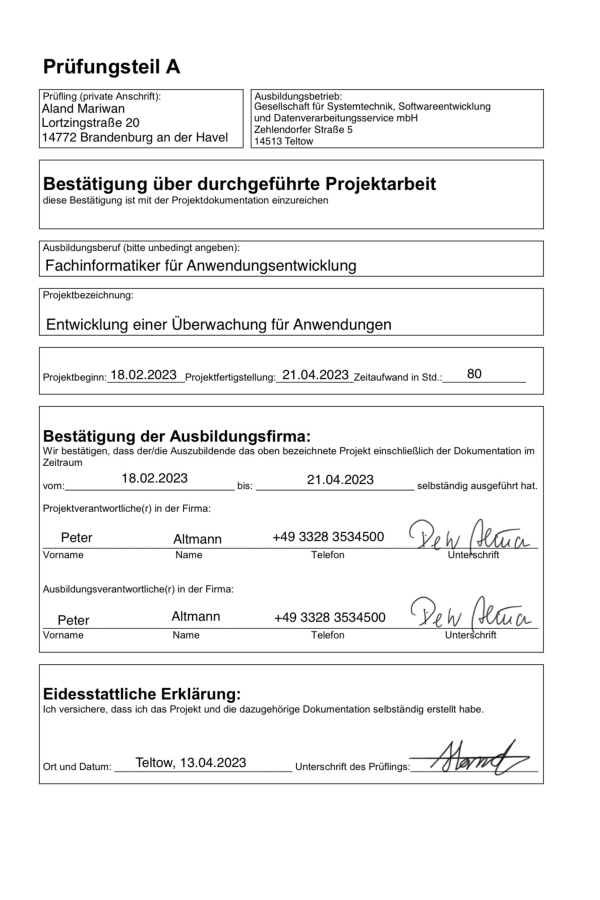
\includepdf[pages=-]{DeckblattIHK.pdf}
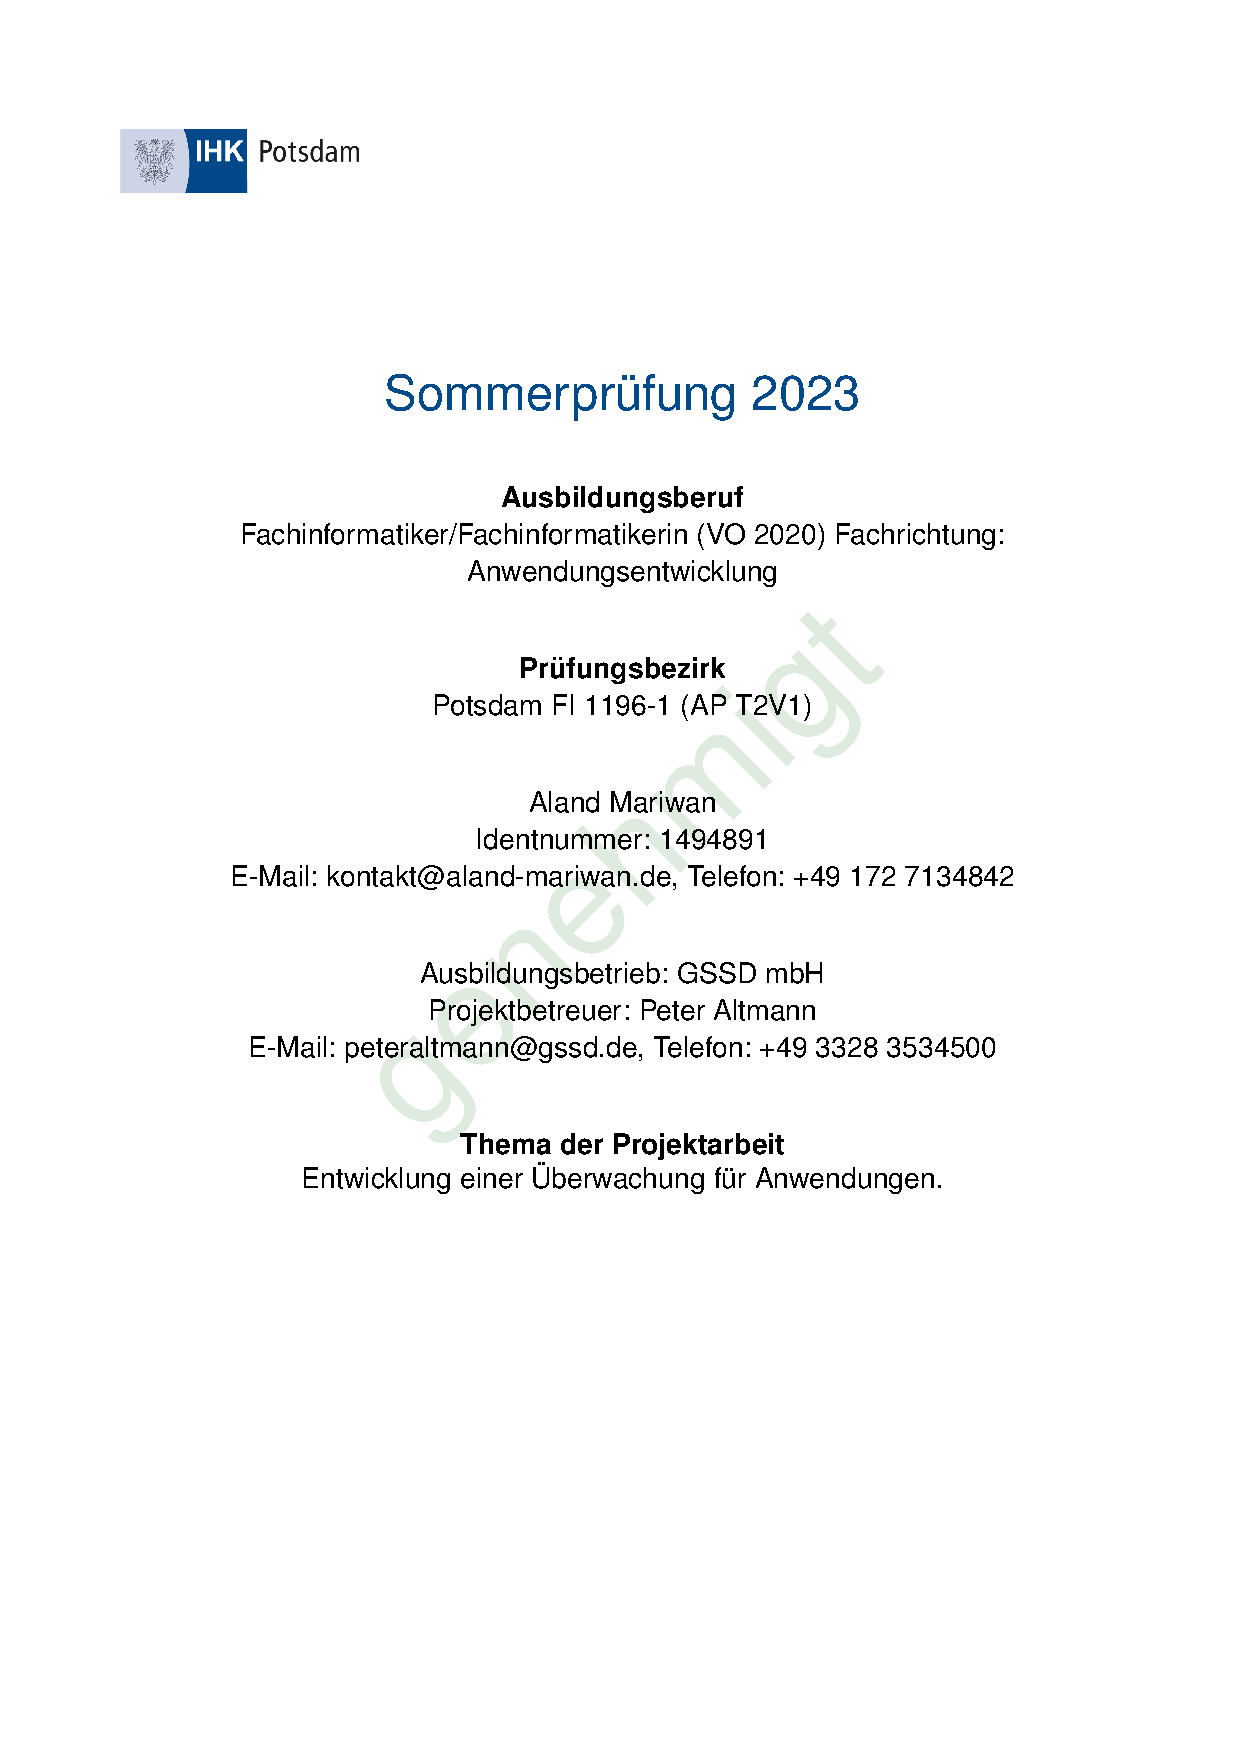
\includepdf[pages=-]{Projektantrag.pdf}
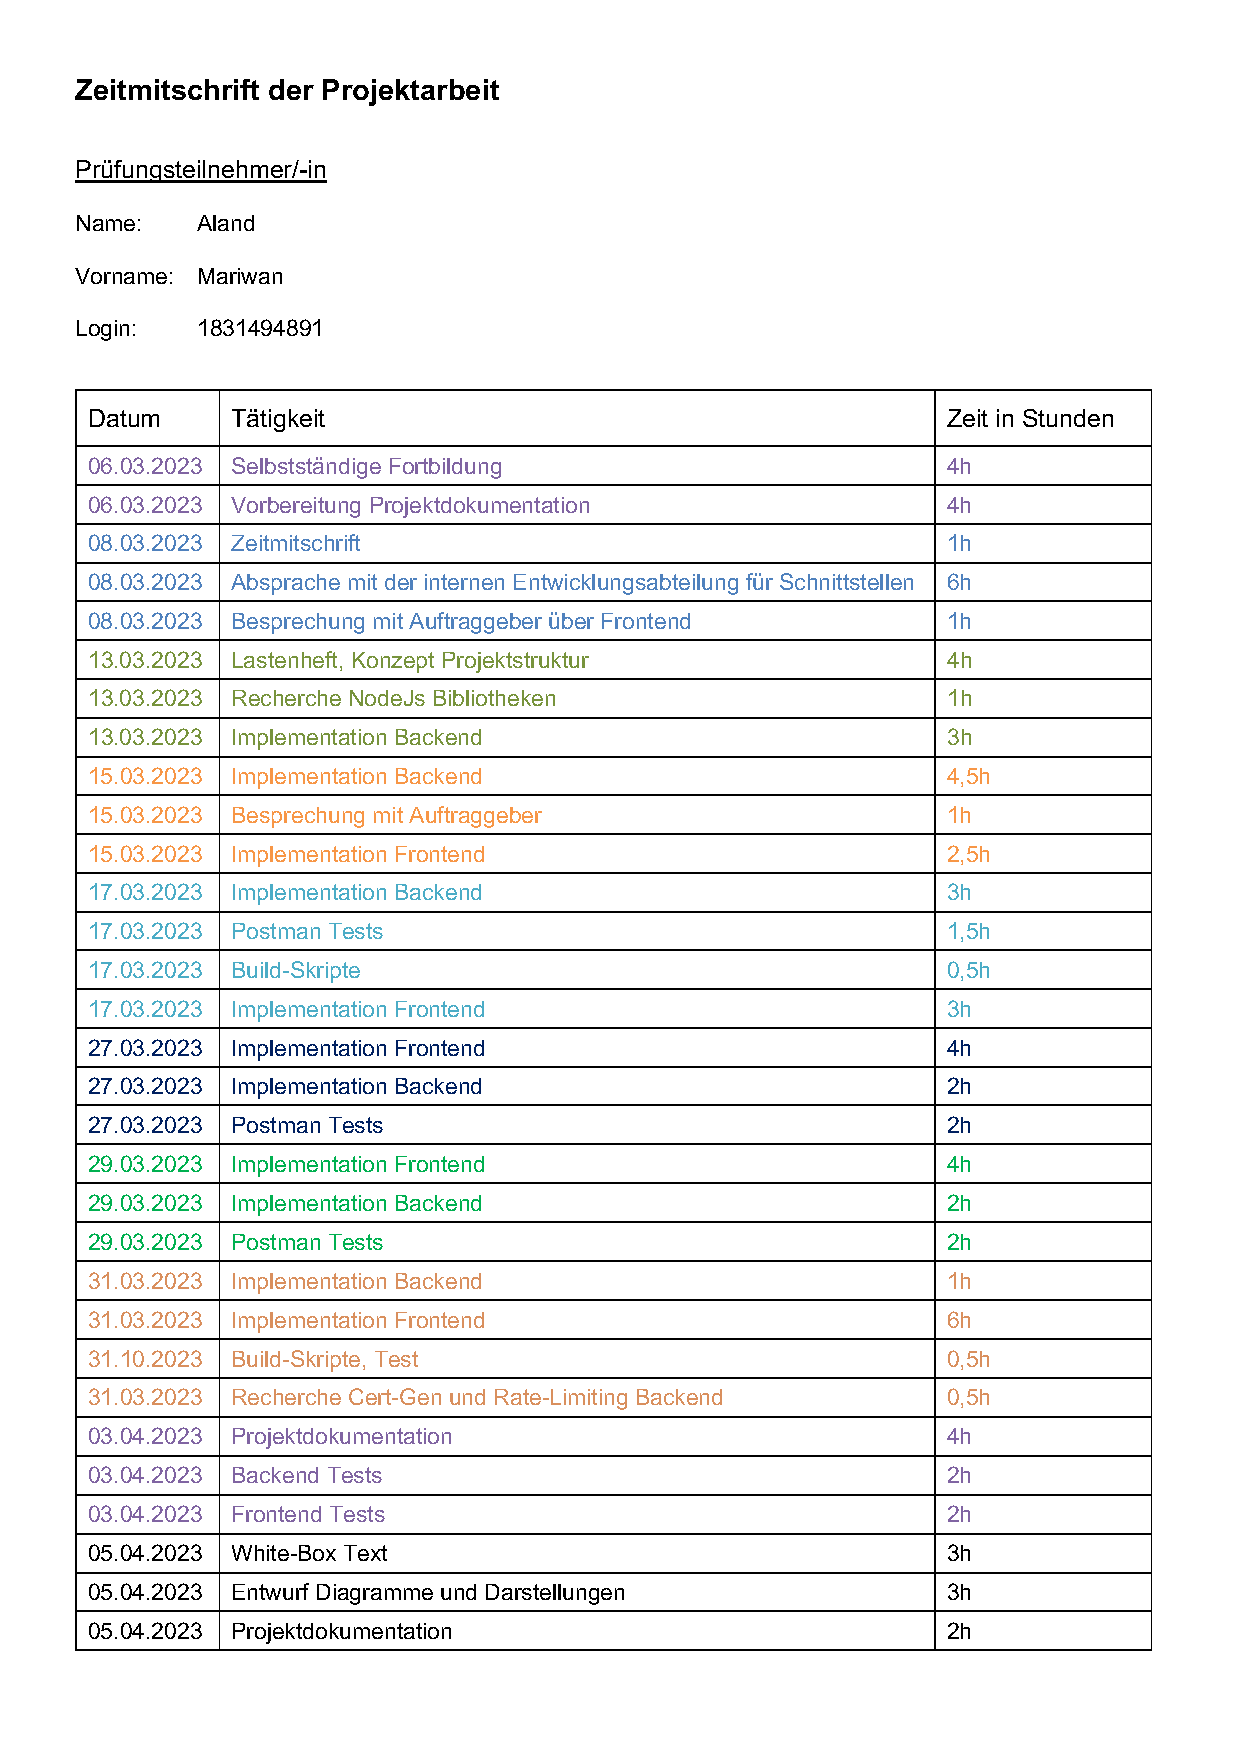
\includepdf[pages=-]{ZeitmitschriftderProjektarbeit.pdf}
\begin{titlepage}
	\centering
	
\includegraphics[width=80mm]{img/ihkpotsdam.png}\\[8ex]
	{\scshape Abschlussprüfung Sommer 2023 \par}
	\vspace{1cm}
	{\scshape Fachinformatikerin für Anwendungsentwicklung\par}
	\vspace{0,5cm}
	{\scshape Dokumentation zur Projektarbeit\par}
	\vspace{1cm}
	{\huge\bfseries {Entwicklung einer Überwachung für Anwendungen}\par}
	\vspace{1cm}

	\begin{center}
	Abgabetermin: Potsdam, den 26.04.2023
	\end{center}
	\vspace{0,5cm}
	\begin{center}
	\small{\textbf{Prüfungsbewerber:}} \\
	\small{Aland Mariwan}\\
	\small{Lortzingstraße 20}\\
	\small{14772 Brandenburg an der Havel}
	\end{center}

	
\includegraphics[width=50mm]{img/main_logo.png}

	\begin{center}
	\small{\textbf{Ausbildungsbetrieb:}} \\
	\small{GSSD mbH}\\
	\small{Zehlendorfer Straße 5}\\
	\small{14513 Teltow}
	\end{center}

\end{titlepage}

\thispagestyle{empty}
\tableofcontents
\listoftables
\listoffigures
\lstlistoflistings
\thispagestyle{empty}
\newpage
{\color{blue}\addsec{Abkürzungsverzeichnis}}

\label{abkuerzungsverzeichnis}
\begin{acronym}[slmtA]
\acro{GSSD}{Gesellschaft für Systemtechnik,Softwareentwicklung und Datenverarbeitungsservice}
\acro{GMS}{GSSD Monitoring System}
\acro{SQL}{Structured Query Language}
\acro{mariaDB}{Maria Database}
\acro{HTML}{Hypertext Markup Language}
\acro{CSS}{Cascading Style Sheets}
\acro{BASH}{Bourne-Again SHell}
\acro{API}{Application Programming İnterface}
\acro{PRs}{Pull Requests}
\acro{REST-API}{Representational State Transfer - Application Programming Interface}
\acro{UML}{Unified Modeling Language}
\acro{CI}{Continuous Integration}
\acro{CD}{Continuous Deployment}
\acro{TDD}{Test-Driven Development}
\acro{BDD}{Behavior-Driven Development}
\acro{IDE}{Integrated Development Environment}
\acro{HTTP}{Hypertext Transfer Protocol}
\acro{HTTPS}{Hypertext Transfer Protocol Secure}
\acro{JSON}{JavaScript Object Notation}
\acro{VSCode}{Visual Studio Code}
\acro{GIT}{Global Information Tracker}
\acro{NPM}{Node Package Manager}
\acro{ERM}{ Entity Relationship Modell}
\acro{MiKTeX}{Mathematical Institute (Mathematisches Institut) (MI) + TeX}
\acro{CDI}{Contexts and Dependency Injection}
\acro{z.B.}{zum Beispiel}
\acro{KI}{künstlicher Intelligenz}
\end{acronym}

\begin{flushleft}
	\setcounter{page}{1}
	\section{Einleitung}
	In dieser Projektdokumentation präsentiert der Autor den Ablauf seines Abschlussprojekts, welches im Rahmen seiner Ausbildung zum Fachinformatiker für Anwendungsentwicklung durchgeführt wurde. Das Projekt fand bei der Gesellschaft für Systemtechnik, Softwareentwicklung und Datenverarbeitungsservice mbH (\acs{GSSD}) in Teltow statt. Aktuell beschäftigt die \acs{GSSD} sieben Mitarbeiter und betreut als IT-Dienstleister zahlreiche kleine und mittlere Unternehmen.
	\\
	Darüber hinaus ist die \acs{GSSD} Partner verschiedener Anbieter von Warenwirtschaftssoftware und offeriert in diesem Bereich Anpassungs- und kundenspezifische Dienstleistungen. Ein weiterer Geschäftszweig der \acs{GSSD} besteht im Verkauf von Hardware für Unternehmen und Privatkunden sowie in der dazugehörigen Installation und Wartung der Systeme.
	\\
	Das Hauptziel dieses Projekts bestand darin, die im Rahmen der Ausbildung erworbenen Kenntnisse und Fähigkeiten anzuwenden und eine webbasierte Anwendung zu entwickeln, die den Anforderungen der \acs{GSSD} gerecht wird. Die Projektdokumentation beschreibt den gesamten Ablauf, von der Planung und Analyse über die Implementierung bis hin zur Bewertung und Dokumentation der Ergebnisse.

	\subsection{Projektbeschreibung}
	Die \acs{GSSD} stellt für einen Kunden ein innovatives Überwachungssystem bereit, das auf dessen Servern laufende Anwendungen, welche als Dienste oder im Hintergrund agieren, effizient überwacht. Das bisherige System lieferte nur ungenügende Informationen, weshalb eine modernere Lösung entwickelt wird, die ein umfassendes Bild der Anwendungslandschaft ermöglicht.
	\\
	Das Herzstück des Projekts ist die Erstellung eines intuitiven Dashboards, das den Anwendungsstatus klar und ansprechend visualisiert. Das Überwachungssystem besteht aus einer leistungsstarken Backend- und einer benutzerfreundlichen Frontend-Anwendung, die es dem Administrator ermöglichen, alle laufenden Anwendungen und deren Interaktionen zu überwachen. Die Anwendungen selbst generieren kontinuierlich Status- und Aktivitätsdaten, die in Datenbanktabellen gespeichert werden. Das Backend verarbeitet diese Daten und bereitet sie für die Darstellung im Frontend auf.
	\\
	Mithilfe von Websockets wird eine nahtlose Kommunikation zwischen Frontend und Backend gewährleistet. Dadurch können Benutzer den Status der Anwendungen jederzeit auf dem Frontend einsehen, solange eine Verbindung besteht. Zudem erlaubt eine intelligente Filterfunktion im Backend, die angezeigten Informationen gezielt zu verfeinern.

	\subsection{Projektziel}
	Das Ziel des Projekts besteht darin, dem Kunden ein ansprechendes Dashboard mit Echtzeit-Visualisierung des Anwendungsstatus zur Verfügung zu stellen,
	um den Administratoren eine umfassende Überwachung der Anwendungen und ihrer Interaktionen zu ermöglichen.
	Die Anwendungen senden kontinuierlich Daten, die vom Backend verarbeitet und in Datenbanktabellen gespeichert werden.
	Die Kommunikation zwischen Frontend und Backend erfolgt über Websockets.
	Die Administratoren haben die Möglichkeit, den Anwendungsstatus abzurufen und neue Sensoren hinzuzufügen.
	Im Falle kritischer Fehler sorgt ein automatisches Benachrichtigungssystem dafür, dass die Administratoren sofort informiert werden und angemessene Maßnahmen ergreifen können.

	\subsection{Projektbegründung}
	Eine effektive Überwachung von Anwendungen und Systemen ist im Bereich der Informationstechnologie von entscheidender Bedeutung, da sie eine frühzeitige Fehlererkennung ermöglicht und negative Auswirkungen auf Betrieb und die Verfügbarkeit minimiert. Ein zuverlässiges Überwachungssystem ermöglicht dem Administrator, die Leistung und den Zustand von Komponenten kontinuierlich zu überwachen, um schnell auf auftretende Probleme zu reagieren. Dadurch werden die Qualität und Verfügbarkeit der Anwendungen verbessert und die Kundenzufriedenheit erhöht.
	\\
	Die Implementierung eines solchen Systems stellt eine reibungslos funktionierende IT-Infrastruktur und eine hohe Kundenzufriedenheit sicher. Mit einem modernen und intuitiven Überwachungssystem können Administratoren potenzielle Probleme frühzeitig erkennen und beheben, bevor sie zu schwerwiegenden Störungen oder Ausfällen führen. Dies trägt dazu bei, den kontinuierlichen Betrieb der Anwendungen und Dienste zu gewährleisten und den Kunden einen zuverlässigen Service zu bieten.

	\subsection{Projektschnittstellen}
	Das Projekt umfasst folgende Schnittstellen:
	\begin{itemize}
	\item Geschäftsführung: Informationen über Projektfortschritte und Entscheidungen, die das Projekt beeinflussen, werden an die Geschäftsführung weitergegeben.
	\item IT-Abteilung: Die IT-Abteilung ist für die technische Umsetzung zuständig und arbeitet eng mit dem Projektteam zusammen.
	\item Externe Dienstleister: Schnittstellen müssen klar definiert werden, um eine reibungslose Zusammenarbeit mit externen Systemen und Dienstleistern zu gewährleisten.
	\item Benutzer: Die Einbindung und Information der Benutzer ist wichtig, um deren Anforderungen gerecht zu werden und eine hohe Akzeptanz des Systems zu erreichen.
	\item Datenbanken und Anwendungen: Die Kommunikation mit anderen Datenbanken und Anwendungen sind erforderlich, um Informationen effizient verarbeiten und austauschen zu können.
	\item Netzwerk- und Sicherheitsinfrastruktur: Schnittstellen zu Netzwerk- und Sicherheitsinfrastruktur müssen definiert werden, um mögliche Anpassungen oder Erweiterungen reibungslos durchführen zu können.
	\end{itemize}


	\subsection{Projektabgrenzen}
	\begin{itemize}
		\item Die Konzeption und Realisierung von Sensoren fällt nicht in den Zuständigkeitsbereich dieses Projekts. Dennoch werden Spezifikationen und Anforderungen definiert, die den Sensoren ermöglichen, sich korrekt an das Backend-System anzubinden.
		\item Schulungen oder Weiterbildungen für Nutzer oder Mitarbeiter sind nicht vorgesehen.
		\item Das Überwachungssystem ist auf ein bestimmtes Team oder eine Abteilung beschränkt, nicht für das gesamte Unternehmen konzipiert.
	\end{itemize}


\subsection{Use-Case}
\subsubsection{Prozessabläufe}
\begin{itemize}
	\item Ablauf 1 beim Überwacher:
	\begin{itemize}
		\item Überwacher öffnet Dashboard.
		\item Dashboard zeigt Anwendungsübersicht und aktuellen Zustand.
		\item Überwacher filtert Anwendungsliste nach Kriterien.
		\item Bewertung jeder Anwendung wird angezeigt.
	\end{itemize}
	\item Ablauf 2 beim Administrator:
	\begin{itemize}
		\item Bei kritischem Zustand oder Problem wird Administrator benachrichtigt.
		\item Administrator reagiert auf Benachrichtigung (Problem lösen, System normalisieren).
		\item Administrator passt Überwachungssystem an, beim Anpassen ist eine Anmeldung erforderlich (Bewertungsfaktoren ändern, Anwendungen hinzufügen oder entfernen).
		\item Administrator öffnet Benachrichtigungseinstellungen im Überwachungssystem.
		\item Administrator konfiguriert Benachrichtigungsschwellenwerte.
		\item Überwachungssystem speichert die Konfiguration und sendet automatisch Benachrichtigungen, wenn Schwellenwerte überschritten werden.
		\item Administrator erhält Benachrichtigungen und ergreift entsprechende Maßnahmen.
	\end{itemize}
		\item Ablauf beim Entwickler
	\begin{itemize}
		\item Entwickler öffnet Sensorintegrationsseite im Überwachungssystem.
		\item Entwickler gibt erforderliche Informationen für den neuen Sensor ein.
		\item Überwachungssystem validiert eingegebene Informationen.
		\item Bei erfolgreicher Validierung wird neuer Sensor dem System hinzugefügt und in der Sensorliste angezeigt.
		\item Bei fehlerhafter Validierung wird Entwickler benachrichtigt und kann die Eingaben korrigieren.
	\end{itemize}
\end{itemize}

\subsubsection{Anwendungsfälle}
Resultierend aus den Prozessabläufen lassen sich die folgende Anwendungsfälle und Abläufe ableiten:
\begin{itemize}
	\item Administratoren/Überwacher als Akteur (Administratoren/Überwacher überwachen Systemzustand und reagieren auf potenzielle Probleme):
	\begin{itemize}
		\item Anmelden im Überwachungssystem
		\item Öffnen von Dashboard
		\item Filtern Anwendungsliste nach Kriterien

	\end{itemize}
	\item Administratoren als Akteur :
		\begin{itemize}
			\item Konfigurieren des Überwachungssystems (Bewertungsfaktoren ändern, Anwendungen hinzufügen oder entfernen)
			\item Öffnen der Benachrichtigungseinstellungen im Überwachungssystem
			\item Konfigurieren Benachrichtigungsschwellenwerte
		\end{itemize}
	\item Entwickler als Akteur (integriert neue Sensoren ins System):
		\begin{itemize}
				\item  Öffnen von Sensorintegrationsseite im Überwachungssystem
				\item  Eingeben der erforderlichen Informationen für den neuen Sensor
		\end{itemize}
\end{itemize}
Das Use-Case-Diagramm ist im Anhang \ref{appendix:a9} auf Seite \pageref{appendix:a9} zu finden.

	\section{Projektplanung}

	\subsection{Projektphasen}
	Im Rahmen des Projektantrags wurden die Projektphasen definiert und in Unterpunkte untergliedert. Für die Durchführung des Projekts stehen insgesamt 80 Stunden zur Verfügung, wobei 20 Stunden für die Planung und Konzeption, 40 Stunden für die Programmierung, 10 Stunden für die Erstellung der Dokumentation und weitere 10 Stunden für die Abnahme des Projekts vorgesehen sind.
	\\
	Eine grobe Zeitplanung wurde vor Beginn des Projekts durchgeführt, um die verfügbare Zeit den jeweiligen Projektphasen zuzuordnen. Diese grobe Zeitplanung ist in Tabelle 1 des Projektantrags dargestellt.

	\subsection{Ressourcenplanung}
	Im Anhang \ref{appendix:a3} werden die verwendeten Ressourcen auf Seite \pageref{appendix:a3}
	aufgelistet, die während des Projekts eingesetzt wurden. Die Planung berücksichtigt
	sowohl Hard- als auch Software-Ressourcen sowie das beteiligte Personal.
	Um Kosten zu minimieren, wurde bei der Auswahl der verwendeten Software darauf geachtet,
	dass keine Lizenzgebühren anfallen, erforderliches Fachwissen vorhanden ist und die
	Architekturrichtlinien der \acs{GSSD} eingehalten werden.
	Die Architekturrichtlinien der \acs{GSSD} legen unter anderem die Nutzung von
	\acs{VSCode} als Entwicklungsumgebung und den Jenkins-Server als Werkzeug für die \acs{CI} fest. Durch die Einhaltung dieser Richtlinien wird sichergestellt,
	dass das Projekt den Anforderungen der \acs{GSSD} entspricht und nahtlos in die bestehende
	Infrastruktur integriert werden kann.

	\subsection{Entwicklungsprozess}
	In der \acs{GSSD} erfolgt die Entwicklung von Kundenprojekten üblicherweise durch den Einsatz der agilen Scrum-Methode. Der Entwicklungsprozess gliedert sich in mehrere ein- oder zweiwöchige Sprints, wobei Github zur Verwaltung der Aufgaben genutzt wird. Die Aufgaben werden den Sprints zugeordnet und während der wöchentlichen Sprintreviews überprüft.\\
Die umgesetzten Aufgaben werden gemeinsam mit dem Projektleiter kontrolliert, getestet und analysiert, um ein effektives Feedback und kontinuierliche Verbesserungen während des gesamten Entwicklungsprozesses zu gewährleisten. Diese strukturierte und kollaborative Vorgehensweise stellt sicher, dass die Endprodukte den Anforderungen und Erwartungen entsprechen.\\

	\section{Analysephase}
	\subsection{Ist-Analyse}
	Der Kunde der \acs{GSSD} verwendet auf seinen Servern verschiedene Anwendungen als Dienste oder im Hintergrund. Zur Überwachung dieser Anwendungen hat der Kunde bereits ein Überwachungssystem im Einsatz. Allerdings erweist sich dieses System als äußerst unzureichend und ineffizient in der Darstellung der Zustände und Informationen, die für die effektive Überwachung der Anwendungen erforderlich sind.
	\\
	Die Ist-Analyse ergab folgende gravierende Schwachstellen im aktuellen Überwachungssystem des Kunden:
	\begin{itemize}
	\item stark eingeschränkte und unvollständige Anzeige von Systemzuständen
	\item mangelhafte Integration und Erkennung von Sensoren, was zu Informationslücken führt
	\item fehlende oder stark verzögerte Benachrichtigungen bei Systemproblemen, wodurch das Eingreifen des Administrators erschwert wird
	\item Schwierigkeiten bei der Skalierbarkeit und Anpassungsfähigkeit an neue Anforderungen, was die Erweiterung und Anpassung des Systems behindert
	\item unübersichtliche und verwirrende Benutzeroberfläche, die eine effiziente Nutzung erschwert
	\item hohe Latenzzeiten und Leistungseinbußen bei der Überwachung von Anwendungen
	\end{itemize}

	Um die Zuverlässigkeit und Funktionalität der überwachten Anwendungen sicherzustellen, müssen diese Schwachstellen dringend angegangen werden. Die Ergebnisse der Ist-Analyse bilden die Grundlage für die anschließende Planung und Implementierung von Verbesserungsmaßnahmen für das Überwachungssystem.
	\subsection{Workflow}

	Der Code definiert sowohl ein Datenmodell als auch einen Sensor mit verschiedenen Eigenschaften wie Name, Typ, Datentyp, Einheit, Minimum- und Maximumwert, Status, Zeitstempel und weiteren Optionen.\\
	Es gibt zwei Arten von Sensoren: echte Sensoren und virtuelle Sensoren. Echte Sensoren senden kontinuierliche Daten an das Backend, während virtuelle Sensoren SQL-Abfragen an das Backend senden, um Daten aus der Datenbank abzurufen.
	\\
	\begin{enumerate}
		\item Der Prozess der Sensorregistrierung beginnt damit, dass der Sensorbauer eine \acs{API}-Anfrage an das Backend sendet und seine Anmeldeinformationen übermittelt. Das Backend prüft, ob der Sensor bereits registriert ist. Wenn nicht, wird der Sensor in der Datenbank registriert und die Anmeldeinformationen werden an den Sensorbauer zurückgesendet.
		\item Nach Erhalt der ID des Sensors kann der Sensor regelmäßig Daten an das Backend übermitteln und Konfigurationsdaten abrufen. Das Backend ruft die Konfigurationsdaten des Sensors über die entsprechende ID aus der Datenbank ab und aktualisiert seine Eigenschaften, wie Name, Typ, Datentyp und Einheit.
		\item Der Sensor kann über die show-Eigenschaft angeben, ob er seine Daten an das Frontend senden und über saveData, ob er seine Daten in der Datenbank speichern möchte. Wenn der Sensor-Daten senden möchte, aktualisiert er das Datenfeld im Sensor-Modell und sendet es an das Backend.
		\item Das Backend prüft, ob die Daten gemäß der in der variablen DataRetentionPeriodInMonths festgelegten Aufbewahrungsfrist gespeichert werden sollen. Wenn der saveData-Wert auf true gesetzt ist, speichert das Backend die Daten in der Datenbank und aktualisiert den Sensor-Status und den Zeitstempel.
		\item Wenn der Sensor ein virtueller Sensor ist, kann er über die commendsql-Eigenschaft SQL-Abfragen an das Backend senden, um Daten aus der Datenbank abzurufen. Das Backend führt die Abfrage aus und sendet das Ergebnis an den virtuellen Sensor.
		\item Das Frontend empfängt die Daten von den aktiven Sensoren und aktualisiert die Benutzeroberfläche entsprechend. Das Backend überwacht den Status der Sensoren und informiert den Sensorbauer über Probleme, die auftreten könnten, wie \acs{z.B.} Sensorausfälle oder Datenbankfehler.
		\item Der Sensorbauer kann über die \acs{API} auch neue Sensoren registrieren, bestehende Sensoren aktualisieren oder löschen sowie weitere Konfigurationen durchführen. Das Backend stellt hierfür entsprechende Funktionen bereit.
	\end{enumerate}
	Das Komponenten Diagramm ist im Anhang \ref{appendix:a10} auf Seite \pageref{appendix:a10} zu finden.



	\subsection{Soll-Konzept}
	In Zusammenarbeit mit Vorgesetzten wurde das folgende Soll-Konzept entwickelt, welches die vom Kunden gestellten Anforderungen an das Überwachungssystem beschreibt.
	Das Überwachungssystem soll alle relevanten Anwendungen auf den Servern des Kunden kontinuierlich überprüfen und bei Fehlererkennung oder Ausfällen den Administrator zuverlässig benachrichtigen. Dabei legt der Kunde Wert auf eine einfache Konfiguration und Verwaltung des Systems.
	Um sicherzustellen, dass das Überwachungssystem den Erwartungen des Kunden gerecht wird, müssen zusätzlich bestimmte Leistungskriterien festgelegt werden. Dazu zählen beispielsweise die maximale Anzahl der zu überwachenden Anwendungen, die Reaktionszeit bei Fehlermeldungen und die Verfügbarkeit des Überwachungssystems.

	\subsection{Risikoanalyse}

Die Analyse möglicher Probleme ist entscheidend, um potenzielle Risiken während der Projektumsetzung zu identifizieren und geeignete Gegenmaßnahmen zu planen. Hier sind die identifizierten Probleme und ihre entsprechenden Risikoanalysen:
	\begin{enumerate}
	\item Integration mit vorhandenen Systemen und Anwendungen,
	\item Datenschutz und Sicherheit,
	\item Skalierbarkeit und Anpassungsfähigkeit,
	\item Kompetenz der beteiligten Mitarbeiter,
	\item Budget- und Zeitbeschränkungen.
	\end{enumerate}
	Durch die frühzeitige Identifizierung dieser potenziellen Probleme und die Umsetzung geeigneter Gegenmaßnahmen können die Risiken während der Projektumsetzung minimiert werden, was zu einer erfolgreichen Implementierung der maßgeschneiderten Überwachungslösung beiträgt.
	\subsection{Wirtschaftlichkeitsanalyse}
	Die Frage, ob sich die Entwicklung dieses Projekts für die \acs{GSSD} lohnt, lässt sich relativ einfach beantworten. Vor Beginn des Projekts wurde der Arbeitsaufwand, unter Berücksichtigung des Tagessatzes, berechnet und dem Kunden ein entsprechendes Angebot unterbreitet. Die im Angebot aufgeführte Vergütung deckt die Projektkosten und erwirtschaftet zusätzlich einen finanziellen Gewinn für das Unternehmen. Eine Wirtschaftlichkeitsanalyse sollte daher die Vorteile des Kunden berücksichtigen. Allerdings gestaltet sich dies schwierig, da dem Autor kritische Daten wie beispielsweise täglicher/monatlicher/jährlicher Zeitaufwand oder Mitarbeiterlöhne des Kunden nicht vorliegen und auch nicht eingeholt werden können. Dennoch kann man davon ausgehen, dass der Kunde die Wirtschaftlichkeit dieser Entscheidung selbstständig berechnet hat und das Ergebnis für zufriedenstellend befunden wurde.

	\subsubsection{„Make or Buy“-Entscheidung}

	Die „Make or Buy“-Entscheidung ist ein wesentlicher Aspekt für Unternehmen, wenn es darum geht, ob sie eine Komponente oder einen Prozess intern entwickeln („Make“) oder von externen Anbietern kaufen („Buy“) sollen. Bei der Entscheidung für ein maßgeschneidertes Überwachungssystem oder eine vorhandene Lösung (\acs{z.B.} Checkmk) sind mehrere Faktoren zu berücksichtigen:

	\begin{itemize} \item \textbf{Kosten:} Die Eigenentwicklung kann hohe Kosten verursachen, während beim Kauf Lizenz- und Supportkosten anfallen. Langfristige Kosteneinsparungen und Effizienz sind jedoch entscheidend.

	\item \textbf{Zeit:} Eigenentwicklungen benötigen mehr Zeit, während der Kauf einer Lösung eine schnellere Implementierung ermöglicht. Anpassungen können jedoch zusätzliche Zeit erfordern.

	\item \textbf{Expertise:} Internes Know-how kann die erfolgreiche Entwicklung eines maßgeschneiderten Überwachungssystems ermöglichen.

	\item \textbf{Anpassungsfähigkeit und Flexibilität:} Eine Eigenentwicklung bietet größere Anpassungsfähigkeit und Flexibilität für unternehmensspezifische Anforderungen.

	\item \textbf{Langfristige Perspektive:} Eine Eigenentwicklung bietet langfristig bessere Kontrolle und Anpassungsfähigkeit, während der Kauf einer Lösung kurzfristige Vorteile bietet.


	\end{itemize}

	Unter Berücksichtigung dieser Faktoren könnte der Kunde zu dem Schluss kommen, dass eine maßgeschneiderte Überwachungslösung langfristig bessere Ergebnisse ermöglicht. Daher wäre die „Make“-Entscheidung für die Entwicklung eines eigenen Überwachungssystems vorzuziehen.

	Der Projektfokus liegt auf der Eigenentwicklung einer maßgeschneiderten Softwarelösung, die den spezifischen Anforderungen und Bedürfnissen des Kunden entspricht. Die Vorteile sind gezielte Gestaltung von Workflow und Benutzerfreundlichkeit, vollständige Kontrolle über Code und Implementierung, effektive Fehlerbehebung und kontinuierliche Verbesserung. Daher ist eine Eigenentwicklung, die ideale Lösung für dieses Projekt.
		\subsubsection{Projektkosten}
		Die Kosten für das Projekt umfassen sowohl Personalkosten als auch sonstige Aufwendungen wie Büroflächen, Stromkosten, Kommunikationskosten usw. Im folgenden ist eine detaillierte Kostenaufstellung für das Projekt dargestellt:
		\begin{itemize}
			\item Personalkosten: Da genaue Personalkosten vertraulich sind, basieren die Berechnungen auf Stundensätzen, die von der Personalabteilung festgelegt wurden. Für Mitarbeiter beträgt der Stundensatz 35,00 €, während der Stundensatz für Auszubildende bei 10,50 € liegt.
			\item Ressourcenkosten: Die Kosten für die in Abschnitt 2.2 (Ressourcenplanung) aufgeführten Ressourcen betragen pauschal 15,00 € über die Projekt-Laufzeit.
			\item Sonstige Aufwendungen: Für Büroflächen, Stromkosten, Kommunikationskosten und weitere allgemeine Kosten wird eine Pauschale von 300,00 € veranschlagt.
		\end{itemize}

		Die Durchführungszeit des Projekts beträgt 80 Stunden. Die untenstehende Tabelle zeigt die Kostenaufstellung, aufgeteilt nach den einzelnen Projektphasen:
			\begin{table}[h]
				\centering
				\begin{tabular}{ >{\bfseries}l l r r r }
					\rowcolor[HTML]{127017}
				\textbf{\color{white}Vorgang} & \textbf{\color{white}Mitarbeiter} & \textbf{\color{white}Zeit} & \textbf{\color{white}kosten pro Stunde} & \textbf{\color{white}Gesamt} \\
				Entwicklungskosten im Rahmen der \acs{GMS} & 1x Auszubildende & 80 & 10,50 & 840,00 \\
				\rowcolor[HTML]{e1efd9}
				Abnahme der Dokumentation & 1x Mitarbeiter & 2h & 35,00 €/h & 70,00 € \\
				Aufsicht bei Projektplanung & 1x Mitarbeiter & 1h & 35,00 €/h & 35,00 € \\
				\rowcolor[HTML]{e1efd9}
				Hilfestellung bei Problemen & 1x Mitarbeiter & 2h & 35,00 €/h & 70,00 € \\
				Pauschalkosten &  &  &  & 315,00 € \\
				\hline
				\rowcolor[HTML]{127017}
				\multicolumn{4}{r}{\textbf{\color{white}Gesamt}} & \textbf{\color{white}1.330,00 €} \\
				\end{tabular}
				\caption{Übersicht der angefallenen Kosten}
				\label{tab:kostenuebersicht}
			\end{table}




		\subsubsection{Amortisationsdauer}
			Die Ermittlung der Amortisationsdauer für den Kunden in diesem Projekt gestaltet sich äußerst komplex, da es weder Vergleichsdaten aufgrund fehlender ähnlicher Anwendungen gibt, noch konkrete Zeitaufwandsangaben vorliegen, wie bereits in Abschnitt 3.2 erwähnt.
			Für die \acs{GSSD} hingegen amortisiert sich das Projekt relativ schnell, da die im Vertrag mit dem Kunden vereinbarten Mitarbeiterstunden in Rechnung gestellt und beglichen werden. Zusätzliche Kosten, die nach der Inbetriebnahme anfallen, wie beispielsweise die Anmietung von Servern zur Bereitstellung der produktiven Anwendung, werden direkt vom Kunden getragen. Daher entstehen für die \acs{GSSD} keine weiteren Kosten, die nicht durch die Zahlungen des Kunden gedeckt wären.

		\subsection{Lastenheft}
			Das Lastenheft beschreibt die Anforderungen an die Überwachung eines komplexen Systems aus Sicht des Kunden.
			Im Anhang \ref{appendix:a1} auf Seite \pageref{appendix:a1} ist das detaillierte Lastenheft des Kunden zu finden.



	\section{Entwurfsphase}

		\subsection{Zielplattform}
			Die zu entwickelnde Lösung ist eine Web-Applikation.
			Das System besteht aus Backend und Frontend, welche über Websockets Daten austauschen.
			Die Datenbank wurde mit \acs{mariaDB} realisiert und enthält Tabellen mit Sensor-Daten und Verwaltungsdaten.
			Das Backend (Node.js, Express) liest und bewertet die Daten und das Frontend (Vue.js) zeigt die ausgewerteten Daten auf dem Dashboard an.

		\subsection{Architekturdesign}
			Das Architekturdesign für die Anwendungsüberwachung besteht aus mehreren Komponenten, die gemeinsam eine umfassende Monitoring-Lösung bieten. Die Architektur beinhaltet das Backend und das Frontend.
			\\
			Das Backend wird in Node.js entwickelt und ist für die Verwaltung der Datenbank und der \acs{API}-Schnittstellen verantwortlich. Es sammelt und analysiert Daten von verschiedenen Anwendungen und speichert sie in der Datenbank. Das Backend verwendet eine \acs{REST-API}, um die Daten an das Frontend weiterzugeben.
			\\
			Das Frontend, das in Vue.js entwickelt wurde, bietet eine grafische Benutzeroberfläche, die den Zustand der Anwendungen visualisiert. Es kommuniziert über WebSocket-Schnittstellen mit dem Backend, um Echtzeitdaten anzuzeigen und interaktive Funktionen wie das Hinzufügen oder Entfernen von Anwendungen sowie das Konfigurieren von Warnmeldungen bereitzustellen.
			\\
			Das Überwachungssystem setzt sich aus Sensoren zusammen, die in jeder Anwendung integriert sind und Daten über deren Leistung und Verfügbarkeit sammeln. Diese Sensoren senden in regelmäßigen Abständen Daten an das Backend, um analysiert und gespeichert zu werden.

		\subsection{Entwurf der Benutzeroberfläche}
			Der Entwurf der Benutzeroberfläche für das Überwachungssystem besteht aus verschiedenen Elementen, um eine intuitive und ansprechende Umgebung für die Benutzer zu schaffen. Hier sind die Hauptkomponenten des Benutzeroberflächenentwurfs:
			\begin{enumerate}
				\item Navigation: Eine Seitenleiste oder ein Menü am seitlichen Rand der Benutzeroberfläche ermöglichen den Benutzern den Zugriff auf verschiedene Abschnitte der Anwendung, \acs{z.B.} Dashboard, Anwendungsverwaltung und Einstellungen.
				\item Dashboard: Das Dashboard ist der zentrale Bereich der Benutzeroberfläche, in dem die aktuellen Statusinformationen der überwachten Anwendungen angezeigt werden. Es kann Kacheln oder Karten enthalten, die für jede Anwendung einen schnellen Überblick über den Zustand, die Leistung und etwaige Warnmeldungen bieten.
				\item Anwendungsverwaltung: In diesem Abschnitt können Benutzer neue Anwendungen hinzufügen, vorhandene Anwendungen entfernen oder konfigurieren und die Sensoren für die Überwachung anpassen.
				\item Einstellungen: Das ist ein Bereich für die Verwaltung von Benutzerkonten, Systemeinstellungen und Benachrichtigungsoptionen.
				\item Filter- und Suchfunktion: Sie bieten eine Möglichkeit für Benutzer, die angezeigten Anwendungen und Daten schnell zu filtern oder nach bestimmten Anwendungen oder Kriterien zu suchen.
				\item Warnmeldungen: Eine Liste oder ein Bereich, der die aktiven Warnmeldungen und kritischen Ereignisse für die überwachten Anwendungen anzeigt. Administratoren können die Warnmeldungen ein- oder ausblenden und Details zu jedem Ereignis anzeigen.
				\item Diagramme und Statistiken: Für jede Anwendung können detaillierte Diagramme und Statistiken zur Leistung und Verfügbarkeit angezeigt werden. Dies kann in Form von Liniendiagrammen, Balkendiagrammen oder Tortendiagrammen erfolgen, je nach Art der Daten und der gewünschten Darstellung.
				\item Responsives Design: Die Benutzeroberfläche sollte so gestaltet sein, dass sie auf verschiedenen Bildschirmgrößen und Geräten gut aussieht und funktioniert, einschließlich Desktop-Computern, Tablets und Mobiltelefonen.
			\end{enumerate}
			Durch die Kombination dieser Elemente wird eine benutzerfreundliche und effektive Benutzeroberfläche geschaffen, die es den Benutzern ermöglicht, die Überwachungsinformationen für ihre Anwendungen leicht zu überprüfen und zu verwalten.

		\subsection{Datenmodell}
			Basierend auf dem Vertrag zwischen der \acs{GSSD} und dem Kunden sowie den zu berücksichtigenden Anwendungsfällen wurde vom Autor die erforderliche Datenbankstruktur analysiert und mithilfe von Node.js-Migrationen erstellt.
			\\
			Diese Datenbankstruktur war auch für die Entwicklung des Frontends von entscheidender Bedeutung, da nahezu jede Entität durch eine eigene Unterseite in der Anwendung repräsentiert wird.
			\\
			Ein vereinfachtes \acs{ERM}, das die Entitäten, Beziehungen und Kardinalitäten zeigt, befindet sich in Anhang \ref{appendix:b} auf Seite \pageref{appendix:b}.

		\subsection{Maßnahmen zur Qualitätssicherung}

			Ein zentrales Element der agilen Entwicklung bei der \acs{GSSD} ist die Durchführung regelmäßiger, technisch fokussierter Meetings. In diesen Sitzungen werden abgeschlossene Arbeitspakete präsentiert, gemeinsam mit dem Projektleiter getestet und gründlich analysiert. Die interdisziplinäre Zusammenarbeit ermöglicht eine fortlaufende Integration der erlangten Erkenntnisse in den Entwicklungsprozess, wodurch die Anwendungsleistung und Codequalität ständig optimiert werden.
			\\
			Die kontinuierliche Qualitätssicherung ermöglicht es, anspruchsvolle Herausforderungen im Entwicklungsprozess effektiv zu bewältigen. Dies resultiert in einer erheblichen Zeitersparnis während der Entwicklung und schafft eine solide Grundlage für eine zukunftssichere und nachhaltige Weiterentwicklung der Anwendung im technischen Bereich.
			\\
			Um die Qualität des Projekts zu gewährleisten, wurden folgende Maßnahmen umgesetzt:
			\begin{enumerate}
				\item \textbf{Unit- und Widget-Tests}: Diese Testverfahren validieren die Richtigkeit der Implementierung und sorgen für eine zuverlässige Funktionalität der Anwendung.
				\item \textbf{Regelmäßige Abstimmungen}: Die Kommunikation mit dem Entwicklungsleiter dient dazu, Abweichungen frühzeitig zu identifizieren und entsprechende Korrekturmaßnahmen einzuleiten.
				\item \textbf{\acs{GIT}-Versionsverwaltung}: Durch den Einsatz von \acs{GIT} wird die Transparenz der Softwareentwicklung gewährleistet.
				\item \textbf{\acs{CI}}: Mithilfe von Jenkins wird nach jedem Push-Vorgang eine automatische Prüfung der Software durchgeführt, um die Qualität ständig zu überwachen und sicherzustellen.
			\end{enumerate}

		\subsection{Deployment} Im Rahmen des Projekts wird die entwickelte Überwachungssoftware auf den Servern des Kunden implementiert und betriebsbereit gemacht. Dabei werden folgende Schritte unternommen:

			\begin{itemize}
				\item Installation der Software: Die entwickelte Anwendung wird auf den vom Kunden bereitgestellten Servern installiert. Dabei werden alle notwendigen Abhängigkeiten und Komponenten eingerichtet.
				\item Konfiguration von Systemeinstellungen: Systemeinstellungen und -parameter werden gemäß den Anforderungen und der Infrastruktur des Kunden angepasst.
				\item Integration mit anderen Anwendungen und Systemen: Die Überwachungssoftware wird mit bestehenden Anwendungen und Systemen des Kunden integriert, um eine nahtlose Zusammenarbeit und Informationsaustausch mit den Sensoren zu gewährleisten.
				\item Durchführung von Tests: Nachdem die Software erfolgreich installiert und konfiguriert wurde, werden Tests durchgeführt, um sicherzustellen, dass sie korrekt funktioniert und keine Fehler oder Probleme auftreten.
				\item Dokumentation: Die Installations- und Konfigurationsprozesse werden dokumentiert, um dem Kunden eine Referenz und Anleitung für zukünftige Anpassungen oder Updates zu bieten.
			\end{itemize}

			Das Deployment der Überwachungssoftware sollte sorgfältig geplant und durchgeführt werden, um mögliche Ausfallzeiten oder Probleme zu minimieren und einen reibungslosen Übergang zu gewährleisten. Hierzu wird ein entsprechender Plan erstellt, der die Aufgaben, Zuständigkeiten und Zeitpläne für das Deployment festlegt. Es werden auch Backup-Pläne und Wiederherstellungsmöglichkeiten eingerichtet, um Datenverluste oder Störungen zu vermeiden.
			\\
			Ein erfolgreicher Abschluss des Deployments stellt sicher, dass das Überwachungssystem effektiv arbeitet und den Kundenbedürfnissen entspricht.


		\subsection{Pflichtenheft}
			Nach Abschluss der Entwurfsphase wurde ein detailliertes Pflichtenheft erstellt, in dem die technischen Lösungen zur Erfüllung der Anforderungen des Lastenhefts dokumentiert sind. Es dient als technische Grundlage für die Implementierungsphase und stellt sicher, dass die umgesetzten Funktionen den Kundenerwartungen entsprechen. Ein Auszug des Pflichtenhefts ist im Anhang \ref{appendix:a2} auf Seite \pageref{appendix:a2} abgebildet.


	\section{Implementierungsphase}


		\subsection{Entwicklung des Dashboards}
			In der Entwicklungsphase des Dashboards lag der Fokus auf der Nutzung von wiederverwendbaren und verschachtelbaren Vue-Komponenten, um eine modulare und erweiterbare Benutzeroberfläche zu schaffen. Das Dashboard besteht aus diversen Komponenten, die spezifische Informationen, wie Benutzerstatistiken, Systemzustand oder Leistungskennzahlen, darstellen. Diese Komponenten wurden auf der Dashboard-Seite integriert, um einen umfassenden und aktuellen Einblick in die Leistung des Überwachungssystems zu ermöglichen.

			Die einzelnen Dashboard-Komponenten wurden so konzipiert, dass sie sowohl autonom als auch in Kombination miteinander funktionieren. Hierbei wurde die Flexibilität von Vue.js genutzt, um die Anordnung und Darstellung der Komponenten dynamisch an die Erfordernisse des Projekts anzupassen. Ein Beispiel hierfür ist die Implementierung von vuetify, einem Material Design Framework für Vue.js, das eine Vielzahl von vordefinierten Komponenten und Layouts bereitstellt.

			Dank der Anwendung asynchroner Funktionen und reaktiver Daten innerhalb der Dashboard-Komponenten werden die dargestellten Informationen kontinuierlich aktualisiert und auf dem neuesten Stand gehalten. Dies ermöglicht die Echtzeitüberwachung verschiedener Systemaspekte und trägt zur raschen Identifizierung von Problemen und Leistungseinbußen bei.

			Im Anhang sind beispielhafte Screenshots des entwickelten Dashboards enthalten, die verschiedene Komponenten und ihre Anordnung innerhalb der Benutzeroberfläche verdeutlichen. Diese Screenshots zeigen, wie das Dashboard eine strukturierte und benutzerfreundliche Visualisierung relevanter Informationen bietet und gleichzeitig flexibel genug ist, um an die spezifischen Anforderungen des Überwachungsprojekts angepasst zu werden.

		\subsection{Datenbank}
			Die verwendete Datenbank für das Projekt ist \acs{mariaDB}. \acs{mariaDB} ist ein weit verbreitetes, relationales Datenbankmanagementsystem, das sich durch seine Skalierbarkeit und Flexibilität auszeichnet. Es ist Open-Source und kann kostenfrei genutzt werden.\\
			Die Integration von \acs{mariaDB} in das Backend ermöglicht die effiziente Verwaltung und Speicherung der gesammelten Daten aus den verschiedenen Anwendungen. Durch die Verwendung von \acs{mariaDB} können auch komplexe Abfragen und Analysen der gespeicherten Daten durchgeführt werden, um wertvolle Erkenntnisse über die Leistung und Verfügbarkeit der überwachten Anwendungen zu gewinnen.\\
			Die Verbindung zwischen dem Backend und der \acs{mariaDB}-Datenbank wird über entsprechende Treiber und Bibliotheken in Node.js hergestellt. Die Datenbankstruktur wird so gestaltet, dass sie leicht erweitert und angepasst werden kann, um neue Anwendungen oder Sensoren hinzuzufügen oder um zusätzliche Funktionen und Warnmeldungen zu unterstützen.\\
			Insgesamt bietet die Verwendung von \acs{mariaDB} als Datenbanklösung für das Projekt eine robuste und skalierbare Grundlage, die den Anforderungen des Kunden gerecht wird und die Möglichkeit bietet, das Überwachungssystem im Laufe der Zeit weiterzuentwickeln und zu optimieren.\\


		\subsection{REST-API}
			In diesem Projekt wird eine \acs{REST-API} verwendet, um den Datenaustausch zwischen den Sensoren und dem Backend zu ermöglichen. Die \acs{REST-API} stellt eine standardisierte und leicht zu verwendende Schnittstelle bereit, um Daten zwischen diesen Systemkomponenten auszutauschen.
			\\
			Die Hauptmerkmale der in diesem Projekt verwendeten \acs{REST-API} sind:
			\begin{enumerate}
				\item Zustandslosigkeit: Jede Anfrage von Client zu Server enthält alle notwendigen Informationen, sodass der Server den Kontext der Anfrage nicht speichern muss. Dies führt zu einer besseren Skalierbarkeit und Vereinfachung der Serverlogik.
				\item Cache-Fähigkeit: Die API-Antworten können gecacht werden, um die Leistung zu verbessern und die Last auf dem Server zu reduzieren.
				\item Client-Server-Architektur: Die \acs{REST-API} trennt die Benutzeroberfläche (Frontend) von der Backend-Logik und der Datenverarbeitung. Dies erlaubt eine unabhängige Entwicklung und Verbesserung der einzelnen Komponenten.
				\item Einheitliche Schnittstelle: Die \acs{REST-API} stellt eine einheitliche und konsistente Schnittstelle bereit, die die Interaktion zwischen den Komponenten vereinfacht.
			\end{enumerate}

			Im Kontext des Projekts werden die Sensoren die \acs{REST-API} verwenden, um Daten an das Backend zu senden oder abzufragen. Das Backend empfängt die Daten von den Sensoren, analysiert und speichert sie in der Datenbank.

			Für die Kommunikation zwischen dem Backend und dem Frontend wird ein Websocket verwendet. Dies ermöglicht eine bidirektionale Kommunikation in Echtzeit zwischen den beiden Komponenten. Das Frontend verwendet den Websocket, um die Daten vom Backend abzurufen und sie in einer benutzerfreundlichen Weise darzustellen.

			Die Verwendung der \acs{REST-API} für die Sensoren und die Websockets für die Kommunikation zwischen Backend und Frontend gewährleistet eine effiziente und zuverlässige Kommunikation, wodurch ein effektives Überwachungssystem für die Anwendungen auf den Servern
			des Kunden geschaffen wird.


		\subsection{Testen der Anwendung}
			Um sicherzustellen, dass die entwickelte Anwendung fehlerfrei funktionierte und die definierten Anforderungen erfüllte, war ein systematischer Testprozess erforderlich. Hierbei kamen verschiedene Testansätze und -ebenen zum Einsatz:

		\begin{enumerate}
		\item Unit-Tests
				\begin{itemize}
					\item Unit-Tests konzentrierten sich auf einzelne Codeeinheiten wie Funktionen oder Klassen. Sie gewährleisteten, dass diese korrekt arbeiteten und die erwarteten Ergebnisse lieferten.
					\item In der Regel wurden Unit-Tests mit Hilfe von Test-Frameworks wie JUnit Mocha (für JavaScript) erstellt und automatisiert ausgeführt.
				\end{itemize}

			\item Integrationstests
				\begin{itemize}
					\item Integrationstests überprüften die korrekte Interaktion zwischen verschiedenen Komponenten der Anwendung, wie zum Beispiel Datenbankzugriffe oder Kommunikation zwischen Backend und Frontend.
					\item Diese Tests wurden sowohl auf Code- als auch auf Systemebene durchgeführt, abhängig von den zu testenden Komponenten.
				\end{itemize}

			\item Systemtests
				\begin{itemize}
					\item Systemtests prüften die Anwendung in ihrer Gesamtheit, um sicherzustellen, dass alle Komponenten ordnungsgemäß zusammenspielten und die Anwendung wie beabsichtigt funktionierte.
					\item Diese Tests umfassten oft auch Last- und Performance-Tests, um die Leistungsfähigkeit und Stabilität der Anwendung unter verschiedenen Bedingungen zu überprüfen.
				\end{itemize}

			\item Akzeptanztests
				\begin{itemize}
					\item Akzeptanztests, auch bekannt als End-to-End-Tests oder Benutzertests, stellten sicher, dass die Anwendung den Anforderungen der Endbenutzer entsprach und alle definierten Use Cases abdeckte.
					\item Diese Tests wurden manuell durchgeführt oder mithilfe von Test-Tools wie Selenium automatisiert, um Benutzerinteraktionen mit der Anwendung zu simulieren.
				\end{itemize}
		\end{enumerate}

			Ein effektiver Testprozess umfasste sowohl manuelle als auch automatisierte Tests und folgte den Prinzipien des \acs{TDD} oder \acs{BDD}, bei denen Tests als integraler Bestandteil des Entwicklungsprozesses betrachtet wurden. Regelmäßige Code-Reviews und die Verwendung von \acs{CI} und \acs{CD} trugen ebenfalls zur Qualitätssicherung der Anwendung bei.

		\subsection{Sicherheitstests}
			Die Sicherheit des Überwachungssystems ist von großer Bedeutung, da es sensible Daten über die überwachten Anwendungen verarbeitet. Daher wurden Sicherheitstests durchgeführt, um potenzielle Schwachstellen und Angriffsvektoren zu identifizieren und entsprechende Gegenmaßnahmen zu implementieren. Dazu zählen unter anderem Tests zur Überprüfung der Authentifizierung, Autorisierung und Verschlüsselung.

	\section{Abnahmephase}

		\subsection{Code-Review}
			Code-Reviews waren ein wesentlicher Bestandteil des Entwicklungsprozesses, um die Codequalität zu gewährleisten und eine kontinuierliche Verbesserung des Codes zu fördern. Sie dienten dazu, potenzielle Fehler frühzeitig zu erkennen und Best Practices für die Codeentwicklung zu fördern.

			Während des Entwicklungsprozesses wurden Code-Reviews durchgeführt, um sicherzustellen, dass:

			\begin{enumerate}
				\item der Code den vereinbarten Programmierstandards und Richtlinien entsprach,
				\item der Code gut strukturiert, lesbar und wartbar ist,
				\item der Code effizient und performant ist,
				\item der Code frei von Sicherheitslücken und Anfälligkeiten ist,
				\item der Code keine unbeabsichtigten Seiteneffekte oder Regressionen verursacht.
			\end{enumerate}

			Um Code-Reviews effektiv zu gestalten, wurden folgende Best Practices angewendet:

			\begin{enumerate}
				\item Die Verwendung von \acs{PRs} in \acs{GIT}, um Änderungen am Code vor der Integration in den Hauptzweig zu überprüfen. Dies ermöglichte es den Entwicklern, Feedback zu geben und Probleme gemeinsam zu lösen.
				\item Die Einhaltung einer Checkliste für Code-Reviews, um sicherzustellen, dass alle wichtigen Aspekte des Codes überprüft wurden.
				\item Die Durchführung von periodischen Code-Reviews mit dem Ziel, mögliche Verbesserungen zu realisieren.
			\end{enumerate}

			Durch das Implementieren dieser Praktiken wurden Code-Reviews zu einem wichtigen Instrument zur Qualitätssicherung und zur Verbesserung des Codes.

		\subsection{Abnahme}
			Im Rahmen dieses Projekts fand keine separate Abnahmephase statt. Stattdessen wurden die Anwendung, ihre Benutzeroberfläche sowie die Interaktion zwischen Frontend und Backend kontinuierlich während des Entwicklungsprozesses in gemeinsamen Sprint-Reviews getestet und besprochen. Durch diesen Ansatz konnte eine interne Abnahme des Projekts bereits während der Entwicklungsphase sichergestellt werden.

			Trotzdem wurde eine formelle Testphase der Benutzeroberfläche, einschließlich JavaScript-Testfällen, durchgeführt. Aufgrund von Verzögerungen kann diese Phase jedoch nicht ausführlich in dieser Projektdokumentation erklärt und berücksichtigt werden.


	\section{Dokumentation}
		Im Rahmen des Projektabschlusses für das spezifische Projekt, das sich auf die Entwicklung einer webbasierten Anwendung für die \acs{GSSD} konzentriert, wurden zwei zentrale Dokumentationen erstellt, um sowohl Endanwendern als auch Entwicklern eine umfassende Informationsquelle zur Verfügung zu stellen. Beide Dokumente wurden fachlich fundiert und ansprechend gestaltet, um ihren jeweiligen Zielgruppen den bestmöglichen Nutzen zu bieten. Im Folgenden werden die spezifischen Ziele und Inhalte dieser Dokumentationen in Bezug auf das Projekt erläutert:


		\subsection{Benutzerhandbuch Endanwender-Dokumentation}

			Das Benutzerhandbuch wurde für die Endanwender der \acs{GSSD} Anwendung konzipiert und bietet eine systematische Einführung in die Plattform, ihre Funktionen und Bedienung. Hierbei wurden ansprechende visuelle Darstellungen und präzise Anweisungen verwendet, um den Anwendern ein effizientes und angenehmes Nutzungserlebnis zu ermöglichen. Das Handbuch enthält detaillierte Schritt-für-Schritt-Anleitungen zur Verwendung der verschiedenen Module und Funktionen der Anwendung, wie \acs{z.B.} Datenverwaltung, Berichterstellung und Zusammenarbeit zwischen verschiedenen Nutzergruppen. Zudem werden Best Practices und nützliche Tipps für den optimalen Einsatz der Software innerhalb der \acs{GSSD} bereitgestellt.

		\subsection{Entwicklerdokumentation}
			Die Entwicklerdokumentation richtet sich an Fachleute, die an der Weiterentwicklung, Wartung oder Integration der \acs{GSSD}-Anwendung beteiligt sind. Diese Dokumentation wurde sorgfältig erstellt, um ein tiefgehendes Verständnis der technischen Aspekte der Software zu vermitteln, einschließlich ihrer Architektur, des Codes, der verwendeten Technologien wie NodeJs, VueJs und \acs{mariaDB} sowie der eingesetzten Bibliotheken und Frameworks. Um den Entwicklern eine strukturierte Orientierungshilfe zu bieten, wurden Best Practices und Richtlinien für die Projektstruktur, das Einrichten der Entwicklungsumgebung, das Durchführen von Tests und das hinzufügen neuer Funktionen integriert. Die Entwicklerdokumentation soll somit eine solide Grundlage für eine effektive Zusammenarbeit und eine qualitativ hochwertige Weiterentwicklung des \acs{GSSD}-Projekts schaffen.


		\section{Fazit}
			Das vom Autor entwickelte Überwachungssystem erfüllt alle im Projektantrag definierten Anforderungen effizient und zuverlässig. Es bietet eine optimale Überwachung der Anwendungen auf den Servern des Kunden. Die identifizierten Schwachstellen des bestehenden Systems werden behoben. Die Anwendungen sind anpassbar und skalierbar, so dass sie mit den Bedürfnissen des Kunden mitwachsen können.
			\\
			Während der Projektdurchführung traten einige Herausforderungen auf, wie \acs{z.B.} die Anpassung des Zeitplans und die Identifizierung der Anforderungen im Lastenheft. Diese wurden jedoch erfolgreich gemeistert und die Erfahrungen können für zukünftige Projekte genutzt werden. Die Zusammenarbeit und Kommunikation mit dem Kunden waren ebenfalls wichtige Aspekte, die während des Projekts berücksichtigt und erfolgreich bewältigt wurden.

		\subsection{Soll-\/Ist-Vergleich}
			Nach Abschluss des Projekts kann festgestellt werden, dass alle im Projektantrag genannten Anforderungen erfolgreich umgesetzt wurden.
			Jedoch musste der Zeitplan im Verlauf des Projekts angepasst werden, da die Umsetzung des Konzepts mehr Zeit in Anspruch nahm als ursprünglich vermutet.
			Die Analyse des Lastenhefts und die Ermittlung der Pflichten waren aufgrund der hohen Anzahl an einzelnen Komponenten und des komplexen Prozesses der Rechtevergabe zeitintensiver als erwartet.
			Die Projektplanungsphase wurde aufgrund der fehlenden Erfahrungen im Vorfeld als aufwendiger eingeschätzt. Die zeitliche Schätzung der weiteren Phasen erwies sich
			insgesamt als zutreffend. Etwa 9 Stunden Arbeitszeit konnten keiner Projektphase direkt zugeordnet werden, da sie für die Überprüfung der Rahmenbedingungen wie das Layout und die Erstellung erforderlicher Anlagen verwendet wurden.

		\subsection{Lessons Learned}
			Während des Projekts wurden verschiedene Erfahrungen gesammelt und wichtige Erkenntnisse gewonnen, die in zukünftigen Projekten genutzt werden können, um den Erfolg und die Effizienz der Projektarbeit zu verbessern. Einige der wichtigsten Lektionen sind:

			\begin{itemize} \item \textbf{Realistische Zeitplanung:} Die Anpassung des Zeitplans während der Projektumsetzung zeigt, wie wichtig es ist, genügend Zeit für die verschiedenen Phasen und Aufgaben einzuplanen. Dabei sollte auch ausreichend Pufferzeit für unvorhergesehene Probleme oder Verzögerungen berücksichtigt werden.
				\item \textbf{Kommunikation und Zusammenarbeit:} Obwohl das Projekt allein durchgeführt wurde, war eine klare Kommunikation mit den Stakeholdern, insbesondere dem Kunden, entscheidend für den Projekterfolg. Regelmäßige Updates und Feedback-Runden stellen sicher, dass alle Anforderungen korrekt verstanden und umgesetzt werden und ermöglichen eine kontinuierliche Verbesserung während des Entwicklungsprozesses.
				\item \textbf{Umfassende Analyse und Dokumentation:} Eine gründliche Analyse der bestehenden Systeme und der Anforderungen des Kunden ist entscheidend für die erfolgreiche Umsetzung eines Projekts. Eine ausführliche und gut strukturierte Dokumentation hilft dabei, den Projektverlauf nachzuvollziehen und eventuelle Probleme oder Verbesserungsmöglichkeiten zu identifizieren.
				\item \textbf{Fehlerbehebung und Tests:} Eine sorgfältige Fehlerbehebung und umfassende Tests während des gesamten Entwicklungsprozesses stellen sicher, dass die entwickelte Lösung den Anforderungen entspricht und funktioniert, wie sie soll. Frühzeitiges Erkennen und Beheben von Fehlern minimiert das Risiko von Problemen in späteren Projektphasen.
				\item \textbf{Anpassungsfähigkeit und Lernbereitschaft:} Die Fähigkeit, sich an Veränderungen oder neue Anforderungen während des Projekts anzupassen, ist entscheidend für den Projekterfolg. Die Bereitschaft, neue Technologien oder Ansätze zu erlernen und anzuwenden, kann dazu beitragen, die Projekteffizienz zu steigern und die Qualität der entwickelten Lösung zu verbessern.
				\item \textbf{Planung für Skalierbarkeit:} Bei der Entwicklung der Überwachungssoftware war es wichtig, die Skalierbarkeit der Lösung zu berücksichtigen, um zukünftige Erweiterungen oder Anpassungen an neue Anforderungen zu ermöglichen. Das Einplanen der Skalierbarkeit reduziert von Anfang an die Wahrscheinlichkeit, dass umfangreiche Änderungen in späteren Projektphasen oder nach der Fertigstellung erforderlich sind.
			\end{itemize}

			Die gewonnenen Erkenntnisse und Lektionen können dazu beitragen, zukünftige Projekte besser zu planen, durchzuführen und abzuschließen, was zu höherer Effizienz, erfolgreichen Projektergebnissen und zufriedenen Kunden führt. Es ist wichtig, diese Lektionen zu dokumentieren und in zukünftigen Projekten zu berücksichtigen, um wiederkehrende Probleme zu vermeiden und die Qualität der Projektergebnisse kontinuierlich zu verbessern.


		\subsection{Ausblick}
			Im Ausblick werden potenzielle Erweiterungen des Systems oder zukünftige Entwicklungen aufgezeigt,
			die auf Kundenfeedback, Marktanforderungen und technologischen Fortschritten basieren.
			Die Integration von \acs{KI} in das System ermöglicht es,
			zukünftige Entwicklungen zu antizipieren und gezielt darauf zu reagieren, um die Wettbewerbsfähigkeit des Systems zu erhalten.
			In diesem Zusammenhang können auch fortgeschrittene Analysemethoden wie Machine Learning und Predictive Analytics eingesetzt werden,
			um Einblicke in Kundenverhalten und Geschäftsentwicklungen zu gewinnen und das System entsprechend zu optimieren.
			Der Ausblick kann auch Informationen über geplante Verbesserungen oder neue Features enthalten,
			die in zukünftigen Releases des Systems implementiert werden sollen und durch den Einsatz von \acs{KI} und anderen fortschrittlichen Technologien unterstützt werden.




	\end{flushleft}


\newpage
{\color{blue}\addsec{Literaturverzeichnis}}

\begin{description}
  \item [NodeJs v18.16.0]
  \item Available at: \url{https://nodejs.org/}
  \item Accessed March 2023
  \item
  \item [expressjs v4.18.2]
  \item Available at: \url{https://expressjs.com/}
  \item Accessed March 2023
  \item
  \item [Mozilla v3]
  \item Available at: \url{https://developer.mozilla.org/}
  \item Accessed March 2023
  \item
  \item [Axios v1.3.5]
  \item Available at: \url{https://axios-http.com/}
  \item Accessed March 2023
  \item
  \item [Vuejs v3]
  \item Available at: \url{https://vuejs.org/}
  \item Accessed March 2023
  \item
  \item [Vuex v3]
  \item Available at: \url{https://Vuex.vuejs.org/}
  \item Accessed March 2023
  \item
  \item [Vuetify v3]
  \item Available at: \url{https://vuetify.org/}
  \item Accessed March 2023
  \item
  \item [Vue Router v3]
  \item Available at: \url{https://router.vuejs.org/}
  \item Accessed March 2023
  \item
  \item [MariaDB v11.1.0]
  \item Available at: \url{https://mariadb.com/}
  \item Accessed March 2023
  \item
  \item [HelmetJs v6.1.5]
  \item Available at: \url{https://helmetjs.github.io/}
  \item Accessed March 2023
\end{description}


\pagenumbering{roman} % Schalte auf römische Seitenzahlen um

\appendix
\section{Anhang}



\subsection{Lastenheft}\label{appendix:a1}\par

Ziel des zu entwickelnden Systems ist die Überwachung eines komplexen Systems, bestehend aus mindestens 10 Komponenten unterschiedlicher Art. Das System soll dem Benutzer ermöglichen, den aktuellen Zustand des Systems auf einen Blick zu bewerten und auf kommende Probleme hinzuweisen.



	\subsubsection{Funktionalitäten}
			Das System soll folgende Funktionalitäten bereitstellen:
		\begin{itemize}
		\item Eine einfache und intuitive Anzeige des Ist-Zustands des Systems, welche eine schnelle und genaue Beurteilung des Systemzustands ermöglicht.
		\item Eine Bewertungsanzeige, welche den Administrator auf kommende Probleme hinweist und eine automatische Alarmierung bei kritischen Zuständen des Systems ermöglicht.
		\item Definition von Schwellwerten für jeden Sensor, um eine effektive Überwachung des Systems zu ermöglichen.
		\item Zusammenfassung der Sensorwerte in einer geeigneten Form, um eine schnelle Bewertung des Systemzustands zu ermöglichen.
		\item Langzeitanalyse der Sensorwerte für Trends und Muster im Systemverhalten.
		\item Interaktive Dashboards für detaillierte Ansichten und individuelle Einstellungen.
		\item Die Sensoren sollen Datenbank-Einträge abfragen. Hilfsprozesse sollen Sensor-Daten in eine Datenbank eintragen, um einen entsprechenden Sensor zu bauen.
		\item Die zeitliche Auflösung der Sensoren muss den erfassten Daten entsprechend angepasst werden können.
		\item Das System soll diskrete Zustandsbeschreibungen bereitstellen. Die Anzeige kann durch verschiedene Darstellungsformen, wie beispielsweise die Größe, erfolgen. Wichtig ist, dass die Anzeige mit einem kurzen Blick zu erfassen ist.
		\item Das System soll einfach zu bedienen und zu warten sein.
		\end{itemize}

		\subsubsection{Technische Anforderungen}

		Das System soll folgende technische Anforderungen erfüllen:

		\begin{itemize}
		\item Das System soll auf einer geeigneten Plattform entwickelt werden, welche eine hohe Verfügbarkeit und Sicherheit gewährleistet.
		\item Die Sensoren sollen über eine geeignete Schnittstelle an das System angeschlossen werden können.
		\item Das System soll die Daten der Sensoren in einer Datenbank speichern.
		\item Das System soll eine Webanwendung sein, die auf einem Server ausgeführt wird.
		\item Das System soll auf einer geeigneten Programmiersprache entwickelt werden, die eine hohe Performance und Skalierbarkeit gewährleistet.
		\item Das System soll auf einem geeigneten Framework aufbauen, welches eine schnelle Entwicklung und Wartung ermöglicht.
		\item Das System soll auf einem geeigneten Betriebssystem ausgeführt werden, welches eine hohe Stabilität und Sicherheit gewährleistet.
		\end{itemize}

		\subsubsection{Nicht-funktionale Anforderungen}

		Das System soll folgende nicht-funktionale Anforderungen erfüllen:

		\begin{itemize}
		\item Das System soll sicher und vor Angriffen geschützt sein.
		\item Das System soll eine hohe Benutzerfreundlichkeit aufweisen, um eine einfache Bedienung zu ermöglichen.
		\item Das System soll eine hohe Zuverlässigkeit aufweisen und bei Ausfällen schnell wiederhergestellt werden können.
		\item Das System soll einfach zu warten und zu aktualisieren sein.
		\end{itemize}

		\subsubsection{Lieferumfang}

		Der Lieferumfang des Projekts umfasst:

		\begin{itemize}
		\item Die vollständige Implementierung des Überwachungssystems.
		\item Eine ausführliche Dokumentation des Systems, einschließlich der Architektur, der Funktionalitäten und der technischen Details.
		\end{itemize}

		\subsubsection{Abnahmekriterien}

		Das Überwachungssystem wird vom Kunden abgenommen, wenn folgende Kriterien erfüllt sind:

		\begin{itemize}
		\item Das System erfüllt alle im Lastenheft definierten Anforderungen.
		\item Das System ist fehlerfrei und stabil.
		\item Das System ist benutzerfreundlich und einfach zu bedienen.
		\item Der Administrator ist in der Lage, das System effektiv zu nutzen.
		\end{itemize}


\clearpage




\subsection{Pflichtenheft}\label{appendix:a2}\par
Das Pflichtenheft definiert die Anforderungen an das zu entwickelnde System und dient als Grundlage für die Umsetzung des Projekts.

\subsubsection{Funktionale Anforderungen}

Das System muss folgende Funktionen bereitstellen:

\begin{enumerate}
\item Übersicht über alle Anwendungen und Systeme beim Kunden
\item Das System muss eine Benutzeranmeldung haben.
\item Das System muss eine Filter funktion für Produkte bereitgestellten.
\item Das System muss eine Sortieren funktion für Produkte bereitgestellten.
\item Generierung von Warnmeldungen, wenn Anwendungen oder Systeme nicht verfügbar sind oder Probleme aufweisen
\item Konfiguration und Anpassung von Warnmeldungen durch Administrator
\item Hinzufügen oder Entfernen von Anwendungen und Systemen durch Administrator
\item Abruf von detaillierten Informationen zu Anwendungen und Systemen, wie z.B. Status, Version, Konfiguration und Abhängigkeiten
\item Starten, Stoppen oder Neustarten von Anwendungen und Systemen durch Administrator
\item Überwachung von Anwendungen und Systemen und Sammlung von Leistungsdaten
\item Erstellung von Berichten über die Verfügbarkeit und Leistung von Anwendungen und Systemen
\item Empfang von Warnmeldungen per E-Mail durch Administrator oder die verantwortliche Person
\item Anpassung der Benutzeroberfläche an die Bedürfnisse der Administrator
\end{enumerate}

\subsubsection{Nicht-funktionale Anforderungen}

Das System muss folgende nicht-funktionale Anforderungen erfüllen:

\begin{enumerate}
\item Sicherheit und Schutz vor Angriffen
\item Hohe Benutzerfreundlichkeit für eine einfache Bedienung
\item Hohe Zuverlässigkeit und schnelle Wiederherstellung bei Ausfällen
\item Einfache Wartung und Aktualisierung
\item Hohe Skalierbarkeit für zukünftiges Wachstum
\end{enumerate}

\subsubsection{Technische Anforderungen}

Das System muss folgende technische Anforderungen erfüllen:

\begin{enumerate}
	\item Plattform
			\begin{itemize}
			\item Das Backend wird mit Node.js implementiert.
			\item Das Frontend wird mit Vue.js implementiert.
			\item Der Mail-Server wird mit \acs{NPM}-Modulen implementiert und muss in der Lage sein, bei Überschreitung bestimmter Schwellenwerte eine E-Mail an die verantwortliche Person zu senden.
			\item Die Webanwendung ist ausschließlich im Intranet erreichbar.
			\item Die Webanwendung wird auf einem Linux-Server innerhalb eines Docker-Containers ausgeführt.
			\item \acs{GIT} wird als System für die Versionskontrolle genutzt.
			\item Github dient als gehostete Softwarelösung für die Versionsverwaltung der \acs{GSSD}.
			\item Der Jenkins-Server ist für die \acs{CD} zuständig.
			\end{itemize}
		\item Datenbank
			\begin{itemize}
				\item Die Datenbankanbindung erfolgt über NodeJs.
				\item Daten, die älter als 6 Monate sind, werden gelöscht.
				\item Die Daten werden in einer MariaDB-Datenbank gespeichert.
				\item Die Repository-Klassen implementieren vorgegebene Interfaces, die die erforderlichen Methoden definieren.
				\item Die Persistenzschicht wird mit Hilfe von Testcontainern getestet.
			\end{itemize}
		\item Backend
			\begin{itemize}
				\item Das Backend muss in der Lage sein, Daten von den Sensoren zu empfangen und zu verarbeiten.
				\item Die verarbeiteten Daten müssen in der Datenbank gespeichert werden.
				\item Es müssen Funktionen implementiert werden, um Warnmeldungen zu generieren und an das Frontend zu senden, wenn bestimmte Schwellenwerte überschritten werden.
				\item Eine zusätzliche Funktion ist erforderlich, um bei Überschreitung bestimmter Schwellenwerte eine E-Mail an die verantwortliche Person zu senden.
				\item Das Benachrichtigungssystem muss einstellbar sein, so dass die verantwortliche Person festlegen kann, welche Schwellenwerte für welche Sensoren überwacht werden sollen und wie die Benachrichtigungen (per E-Mail, Push-Benachrichtigung an Frontend) bei Überschreitung dieser Schwellenwerte gesendet werden sollen.
			\end{itemize}

		\item Benutzeroberfläche
			\begin{itemize}
				\item Die Benutzeroberfläche muss über WebSocket-Schnittstellen auf das Backend zugreifen, um aktuelle Daten in Echtzeit anzuzeigen.
				\item Die Benutzeroberfläche muss interaktive Funktionen bereitstellen, die es Benutzern ermöglichen, Anwendungen hinzuzufügen oder zu entfernen sowie Warnmeldungen einzustellen.
				\item Die WebSocket-Schnittstellen müssen sicher und robust sein, um eine zuverlässige Kommunikation zwischen Frontend und Backend zu gewährleisten.
				\item Die Benutzeroberfläche muss in Vue.js entwickelt werden, um eine reibungslose Integration mit dem Backend zu gewährleisten.
				\item Eine barrierefreie Gestaltung sollte bei der Entwicklung der Benutzeroberfläche berücksichtigt werden.
				\item Die Benutzeroberfläche muss in Übereinstimmung mit der Corporate Identity der \acs{GSSD} gestaltet werden und die aktuellen Designrichtlinien einhalten.
				\item Die Benutzeroberfläche muss getestet werden, um sicherzustellen, dass sie ordnungsgemäß funktioniert und eine benutzerfreundliche Erfahrung bietet.
				\item Die Benutzeroberfläche muss mit modernen Browsern kompatibel sein und sich an verschiedene Bildschirmgrößen anpassen können.
				\item Die Benutzeroberfläche muss eine Seite bereitstellen, auf der das Benachrichtigungssystem konfiguriert werden kann. Auf dieser Seite sollten Optionen zur Verfügung stehen, um festzulegen, welche Schwellenwerte für Warnmeldungen aktiviert sein sollen und welche Benutzer für diese Meldungen benachrichtigt werden sollen. Es sollte auch möglich sein, die bevorzugte Methode der Benachrichtigung (z.B. E-Mail, Push-Benachrichtigung) für jeden Benutzer einzustellen. Die Benutzeroberfläche sollte benutzerfreundlich gestaltet sein und es dem Benutzer einfach machen, die gewünschten Einstellungen vorzunehmen.
			\end{itemize}
		\item Geschäftslogik
			\begin{itemize}
				\item Zur Erzeugung von Objekten wird \acs{CDI} verwendet.
				\item Das Framework JUnit 5 wird für automatisierte Tests eingesetzt.
				\item Das Frontend stellt eine Benutzeroberfläche bereit, um Daten an das Backend zu übermitteln.
				\item Das Frontend empfängt Daten vom Backend und stellt sie in der Benutzeroberfläche dar.
				\item Das Frontend stellt Funktionen bereit, um Warnmeldungen zu generieren und an das Backend zu senden, wenn bestimmte Schwellenwerte überschritten werden.
			\end{itemize}
\end{enumerate}

\subsubsection{Lieferumfang}

Der Lieferumfang des Projekts umfasst:

\begin{enumerate}
\item Vollständige Implementierung des Systems
\item Ausführliche Dokumentation des Systems, einschließlich Architektur, Funktionalitäten und technischer Details
\end{enumerate}

\subsubsection{Abnahmekriterien}

Das System wird vom Kunden abgenommen, wenn folgende Kriterien erfüllt sind:

\begin{enumerate}
\item Erfüllung aller im Pflichtenheft definierten Anforderungen
\item Fehlerfreiheit und Stabilität des Systems
\item Benutzerfreundlichkeit und einfache Bedienung des Systems
\item Effektive Nutzung des Systems durch die Benutzer
\end{enumerate}



\clearpage



\subsection{Verwendete Ressourcen}\label{appendix:a3}\par
 Hardware
	\begin{itemize}
		\item Laptop
		\item Büroeigener Server – Bereitstellung der Testumgebung
	\end{itemize}

Software
	\begin{itemize}
		\item Figma -- Programm zur Erstellung von Mockups
		\item \acs{VSCode} -- Code Editor
		\item NodeJs -- plattformunabhängige JavaScript-Laufzeitumgebung
		\item \acs{NPM} – Package Manager für das Projekt
		\item VueJS -- JavaScript-Framework für Benutzeroberflächen
		\item \acs{VSCode} mit \acs{MiKTeX} -- Entwicklungsumgebung für \LaTeX
		\item Draw.io – Website zum Erstellen von Diagrammen
		\item Lucidchart – Website zum Erstellen von Diagrammen
		\item \acs{GIT} -- Verteilte Versionsverwaltung
		\item Jenkins -- Buildserver
		\item Postman -- Test und Dokumentation von \acs{REST-API}s
		\item JUnit -- Framework zur Durchführung von Unit-Tests
		\item \acs{MiKTeX} -- Distribution des Textsatzsystems \TeX
		\item Mockito -- Mocking-Framework zur Erstellung von Pseudoklassen
		\item \acs{mariaDB} -- Datenbanksystem
		\item Github -- Projektmanagement
		\item Windows 10 -- Betriebssystem
		\item Ubuntu Server 22.04 -- Betriebssystem
		\item Internet Browser (Firefox, Chrome, IE) – Darstellung der lokalen Umgebung und Zugang
	auf das Testsystem
	\end{itemize}

 Personal
	\begin{itemize}
		\item Auszubildender -- Umsetzung des Projektes
		\item Entwickler, Projektleiter – Umsetzung des Backends der Applikation und Review des Codes
		\item Geschäftsführer – Beratung, Hilfe bei Fragestellungen, Kommunikation mit dem Kunden
	\end{itemize}
Sonstiges
	\begin{itemize}
		\item Büro
		\item Arbeitsplatz
	\end{itemize}
\clearpage




\begin{table}[htbp]
	\centering
	\begin{tabular}{ l l }
	\hline
	\rowcolor[HTML]{127017}
	\textbf{\color{white}Tätigkeit} & \textbf{\color{white}Zeit in Stunden} \\
	Selbstständige Fortbildung & 4h \\
	Vorbereitung Projektdokumentation & 4h \\
	Zeitmitschrift & 1h \\
	Absprache mit der internen Entwicklungsabteilung für Schnittstellen & 6h \\
	Besprechung mit Auftraggeber über Frontend & 1h \\
	Lastenheft, Konzept Projektstruktur & 4h \\
	Recherche NodeJs Bibliotheken & 1h \\
	Implementation Backend & 3h \\
	Implementation Backend & 4,5h \\
	Besprechung mit Auftraggeber & 1h \\
	Implementation Frontend & 2,5h \\
	Implementation Backend & 3h \\
	Postman Tests & 1,5h \\
	Build-Skripte & 0,5h \\
	Implementation Frontend & 3h \\
	Implementation Frontend & 4h \\
	Implementation Backend & 2h \\
	Postman Tests & 2h \\
	Implementation Frontend & 4h \\
	Implementation Backend & 2h \\
	Postman Tests & 2h \\
	Implementation Backend & 1h \\
	Implementation Frontend & 6h \\
	Build-Skripte, Test & 0,5h \\
	Recherche Cert-Gen und Rate-Limiting Backend & 0,5h \\
	Projektdokumentation & 4h \\
	Backend Tests & 2h \\
	Frontend Tests & 2h \\
	White-Box Text & 3h \\
	Entwurf Diagramme und Darstellungen & 3h \\
	Projektdokumentation & 2h \\
	\end{tabular}
	\caption{Detaillierte Zeitmitschrift}
	\label{tab:zeitaufwand}
	\end{table}
\clearpage

\subsection{Middleware}\label{appendix:a5}\par
Middleware bezeichnet eine Art von Anwendungssoftware, die als Vermittler zwischen verschiedenen Systemen oder Komponenten fungiert. Es handelt sich um eine Funktion, die Zugriff auf den Anfrage-Antwort-Zyklus der Anwendung hat. Middleware kann dabei helfen, den Ablauf von Anfragen und Antworten zu steuern, indem sie Daten von der Anfrage entgegennimmt und an die Anwendung weiterleitet, sowie die Antwort von der Anwendung entgegennimmt und an den Client zurücksendet.
\\
\begin{figure}[htbp]
	\centering
	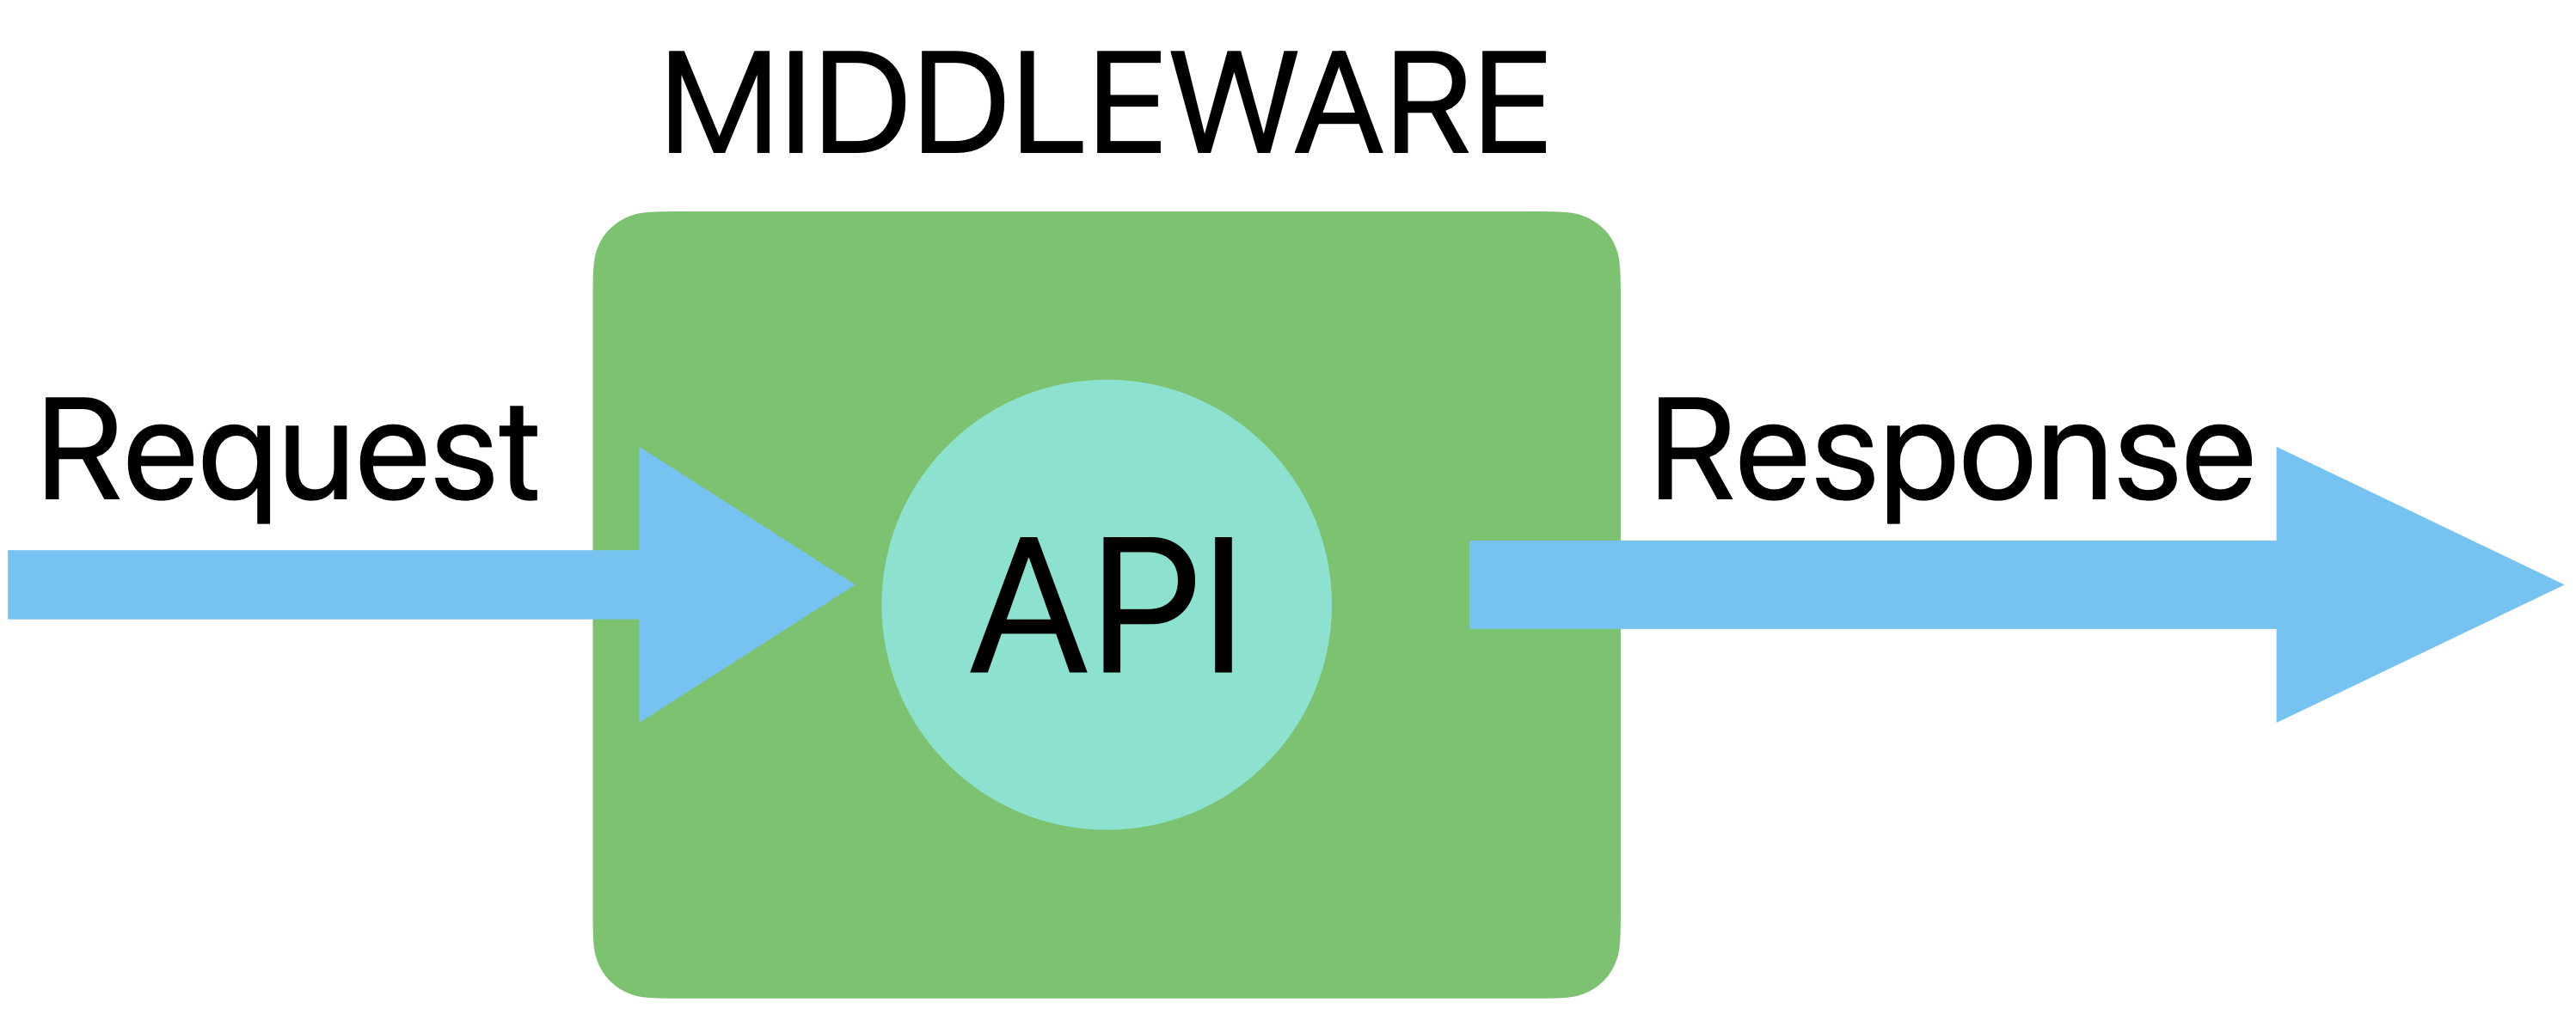
\includegraphics[width=250px]{img/ExpressJS_Middleware_1.png}
	\caption{ExpressJS Middleware}
\end{figure}
Eine Middleware-Funktion enthält in der Regel das Anfrageobjekt, das Antwortobjekt und die Middleware-Funktion selbst. Middleware kann auch die Antwort an den Server senden, bevor die Anfrage abgeschlossen ist. Die nächste Middleware-Funktion wird normalerweise als Variable mit dem Namen "next" dargestellt. Im Grunde ist Middleware eine Funktion, die nur über Routen angewendet werden kann. Middleware kann auch verwendet werden, um auf Anfragen und Antworten zuzugreifen und diese zu ändern.
\\
Middleware kann mehrere Aufgaben erfüllen. Es kann beliebigen Code ausführen, Änderungen an den Anfrage-Antwort-Objekten vornehmen, den Anfrage-Antwort-Zyklus beenden oder die nächste Middleware-Funktion im Stapel aufrufen. Mit diesen Funktionen können wir Middleware modifizieren, um viele Aufgaben auszuführen, wie beispielsweise eine Website für bestimmte Länder zu sperren oder die Authentifizierung eines Benutzers zu überprüfen.
\\
Um Middleware in einer Express-Anwendung zu erstellen, können wir eine separate Middleware-Datei erstellen und diese ausführen. Dazu müssen wir zunächst alle Pakete installieren, die für die Ausführung von Express-Middleware benötigt werden. Anschließend können wir die Middleware-Datei erstellen und ausführen, um die Funktionen der Middleware in unserer Anwendung zu nutzen.
\\
Im Beispiel wird gezeigt, wie eine Middleware-Funktion in Express erstellt werden kann. Zunächst wird eine einfache Express-\acs{API} erstellt und dann eine Middleware-Datei erstellt. In dieser Datei wird die Middleware-Funktion definiert, die aufgerufen wird, wenn eine Anfrage an die \acs{API} gestellt wird. Die Middleware-Funktion ruft dann die nächste Middleware-Funktion auf und gibt die Antwort an den Client zurück.
\\
Insgesamt bietet Middleware eine einfache Möglichkeit, um verschiedene Funktionen in eine Anwendung zu integrieren und diese zu verwalten. Durch die Verwendung von Middleware können Entwickler schnell und einfach Funktionen hinzufügen oder entfernen, um die Funktionalität ihrer Anwendungen zu verbessern.

\subsection{Der Grund für die Verwendung von Session}\label{appendix:a6}\par
In der Webentwicklung ist die Verwendung von Sessions ein wichtiger Aspekt bei der Entwicklung von Überwachungssystemen. Eine Session ermöglicht es, den Benutzer während seiner Interaktion mit dem System zu identifizieren und seine Aktionen zu verfolgen. Dies ist besonders wichtig bei der Überwachung eines komplexen Systems, bei dem viele Komponenten beteiligt sind.
\\
Durch die Verwendung von Sessions kann der Benutzer authentifiziert werden, um sicherzustellen, dass nur autorisierte Benutzer auf das System zugreifen können. Außerdem kann die Session genutzt werden, um die Berechtigungen des Benutzers zu überprüfen und sicherzustellen, dass er nur auf die Bereiche des Systems zugreifen kann, auf die er zugreifen sollte.
\\
Eine Session ermöglicht auch die Verfolgung der Aktivitäten des Benutzers im System, was hilfreich sein kann, um ungewöhnliches Verhalten oder mögliche Sicherheitsbedrohungen zu erkennen. Durch die Aufzeichnung von Benutzeraktivitäten in der Session können Probleme schneller erkannt und behoben werden.

\subsection{Der Grund für die Verwendung von Helmet.js}\label{appendix:a7}\par
Helmet.js ist ein Middleware-Modul für Express, das verschiedene \acs{HTTP}-Header für verbesserte Sicherheit konfiguriert. Es ist wichtig für die Webentwicklung, insbesondere für Systeme zur Überwachung, da es dazu beiträgt, Angriffe auf die Anwendung zu verhindern und die Sicherheit zu erhöhen. Einige der Funktionen, die Helmet.js bietet, sind:
\begin{itemize}
	\item \textbf{XSS-Schutz:} Cross-Site-Scripting-Angriffe können durch Einfügen von Skripten in die Benutzereingabe durchgeführt werden. Helmet.js konfiguriert den X-XSS-Protection-Header, um solche Angriffe zu blockieren.
	\item \textbf{HTTP-Header-Steuerung:} \acs{HTTP}-Header können so konfiguriert werden, dass sie Angriffe verhindern oder abmildern. Beispielsweise kann der X-Content-Type-Options-Header so eingestellt werden, dass der Browser dazu gezwungen wird, nur MIME-Typen zu akzeptieren, die der Server ausdrücklich angibt.
	\item \textbf{Clickjacking-Schutz:} Clickjacking-Angriffe können dazu führen, dass Benutzer auf unerwünschte Links klicken, ohne es zu merken. Helmet.js konfiguriert den X-Frame-Options-Header, um solche Angriffe zu verhindern.
	\item \textbf{Weitere Funktionen:} Weitere Funktionen von Helmet.js sind das Verhindern von MIME-Sniffing, das Verbergen von X-Powered-By-Headern und das Hinzufügen von Strict-Transport-Security-Headern.
\end{itemize}

\clearpage

\subsection{Fehlercodes und Statuscode-Meldungen}\label{appendix:a8}\par
In der Webentwicklung ist es von großer Bedeutung,
standardisierte Fehlercodes und Statuscode-Meldungen zu verwenden, da sie dazu beitragen, Fehler schnell zu erkennen und zu beheben. Eine Tabelle, die diese Codes und Meldungen enthält (siehe Abbildung 2), ist eine nützliche Referenz, um Fehler zu identifizieren und zu beheben. Die Tabelle sollte alle relevanten Codes enthalten, die von der Anwendung verwendet werden, sowie eine kurze und klare Beschreibung der zugehörigen Meldungen. Es ist auch wichtig, dass die Codes und Meldungen präzise formuliert sind, um eine einfache Verständlichkeit zu gewährleisten.
\begin{figure}[htbp]
	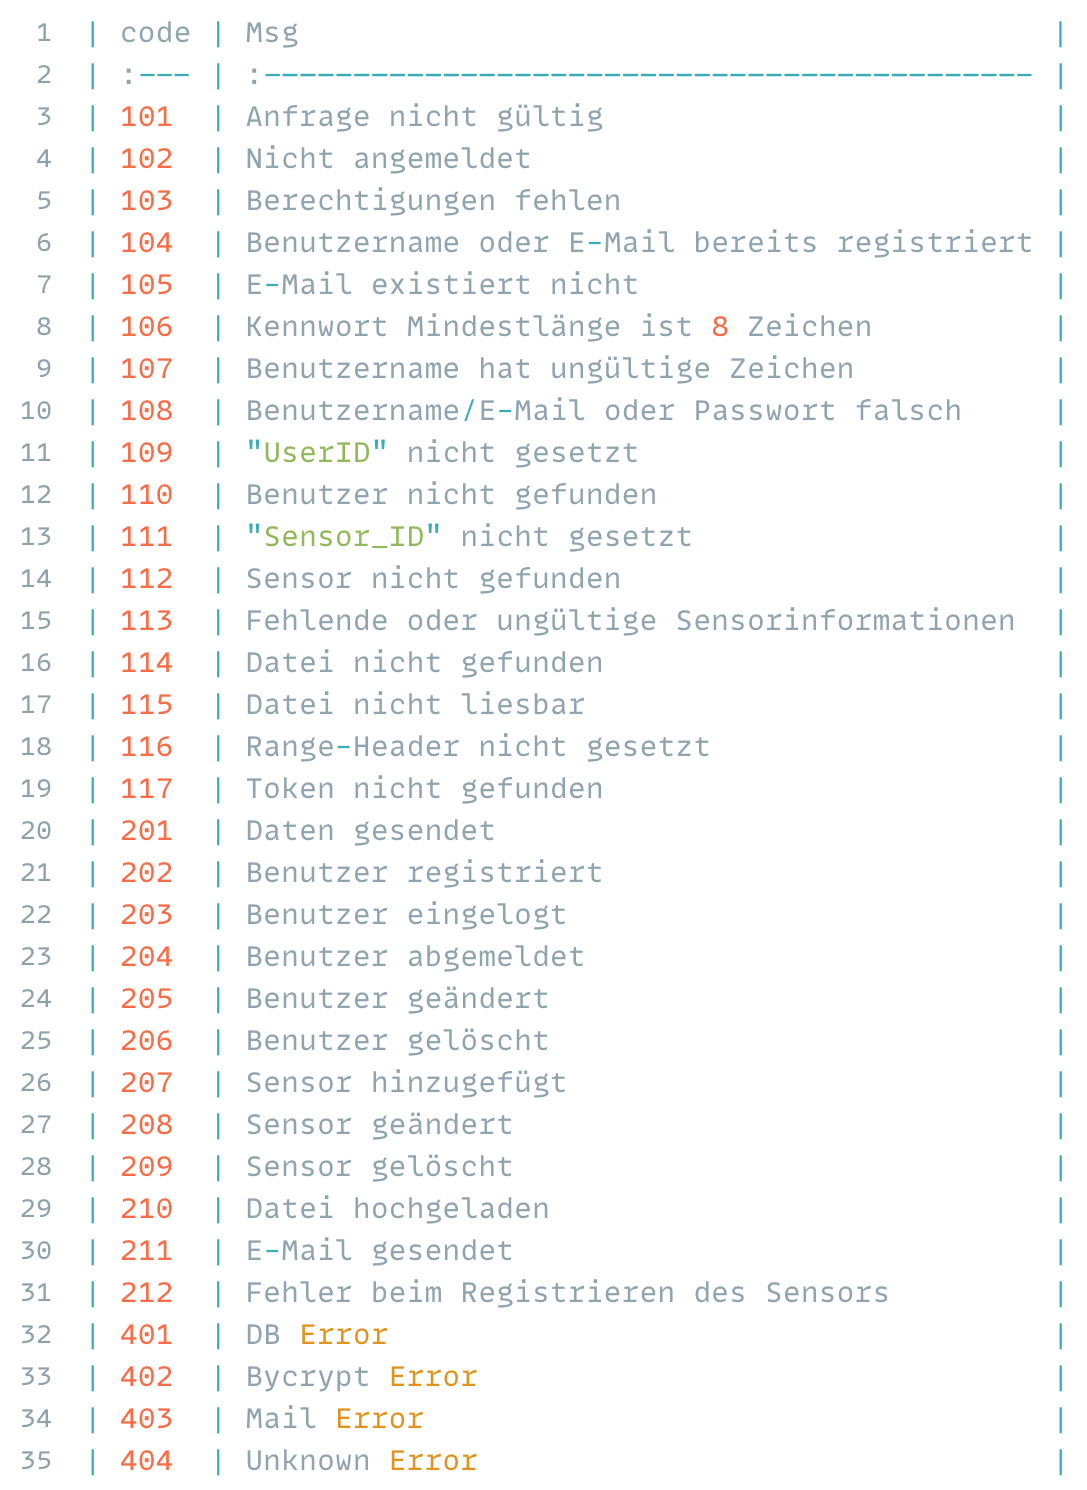
\includegraphics[width=300px]{img/Statuscode-Meldungen.png}
	\caption{Fehlercodes und Statuscode-Meldungen}
\end{figure}

\clearpage

\subsection{Use-case Diagramm}\label{appendix:a9}\par
\begin{figure}[htbp]
	\centering
	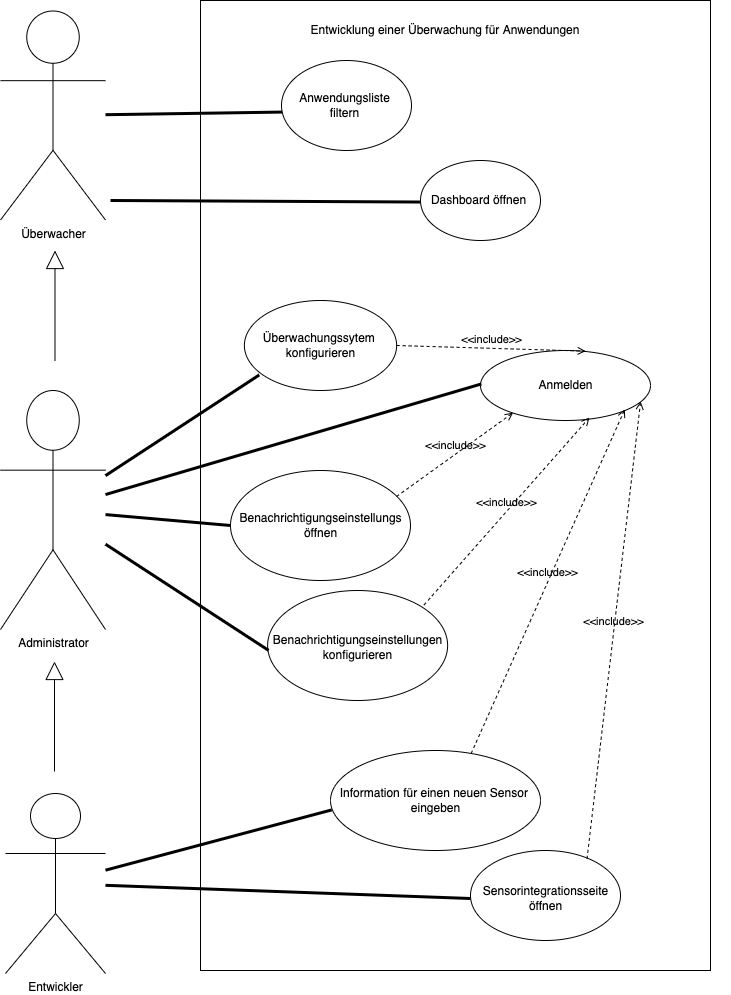
\includegraphics[width=300px]{img/anwendungsfalldiagramm.png}
	\caption{Use-case Diagramm}
\end{figure}
\clearpage



\subsection{Komponenten Diagramm}\label{appendix:a10}\par
\begin{figure}[htbp]
	\centering
	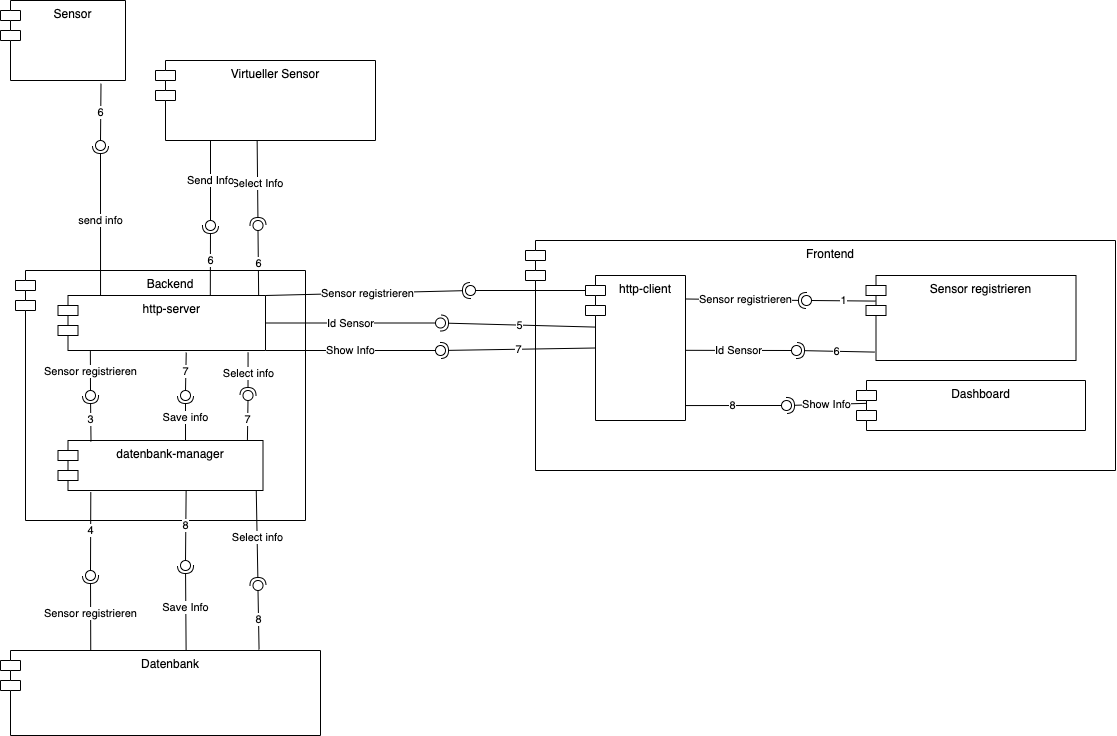
\includegraphics[width=1\textwidth]{img/komponent_diagram.png}
	\caption{Komponenten Diagramm}
\end{figure}
\clearpage

\section{Relationales Datenbankmodell}\label{appendix:b}\par

Für dieses Projekt wurde ein Entity-Relationship-Diagramm (ER-Diagramm) erstellt, um die Struktur der Datenbank und die Beziehungen zwischen den verschiedenen Entitäten zu modellieren. Das ER-Diagramm bildet die Grundlage für das Datenbankschema und hilft bei der Organisation der Daten, die im Rahmen des Überwachungssystems erfasst und verarbeitet werden.
\begin{figure}[h]
	\centering
	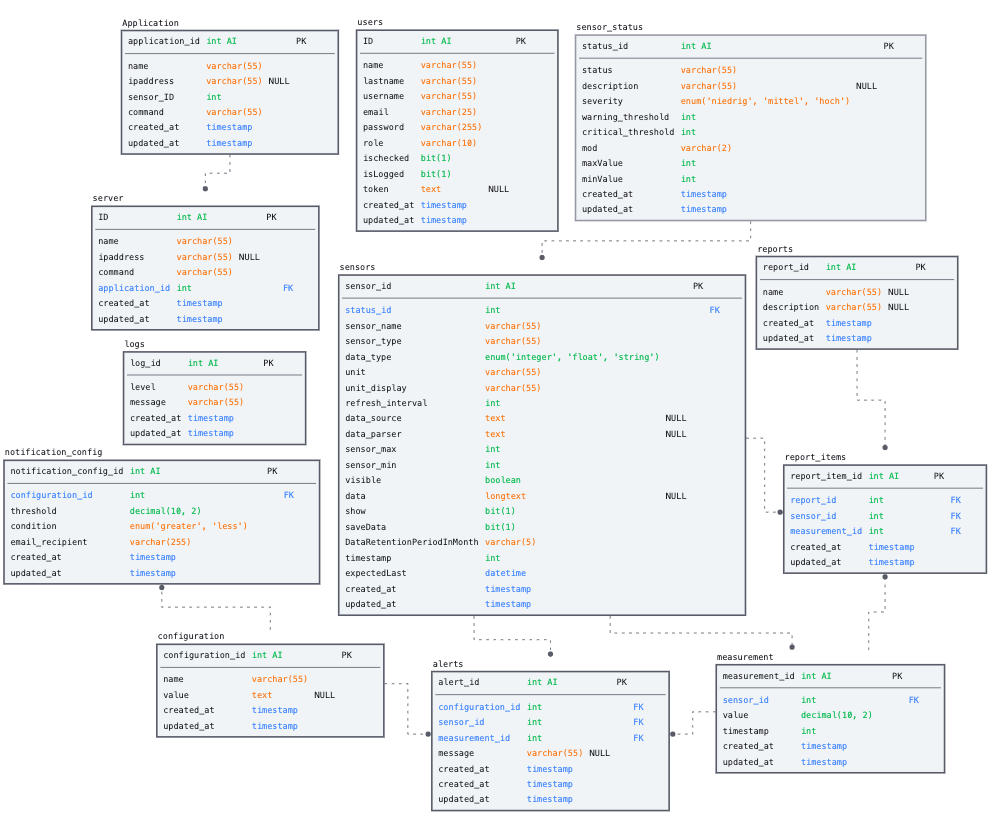
\includegraphics[width=1\textwidth]{img/ERP-diagramm.png}
	\caption{Relationales Datenbankmodell}
	\label{Relationales Datenbankmodell}
\end{figure}
\clearpage

\subsection{Screenshot des Sprint-Boards in GitHub}\label{appendix:b1}\par


In diesem Projekt wurde ein Sprint-Board in GitHub für die Planung und Verwaltung der Softwareentwicklung eingesetzt. Das Kanban Board ermöglichte eine effektive Organisation der verschiedenen Aufgaben und Phasen des Projekts, indem es den Fortschritt in Echtzeit darstellte. Als Einzelperson war das Kanban Board ein wertvolles Instrument zur Selbstorganisation und zum Nachverfolgen der Aufgaben, um sicherzustellen, dass alle notwendigen Schritte abgeschlossen und Ziele erreicht wurden.

\begin{figure}[htbp]
	\centering
	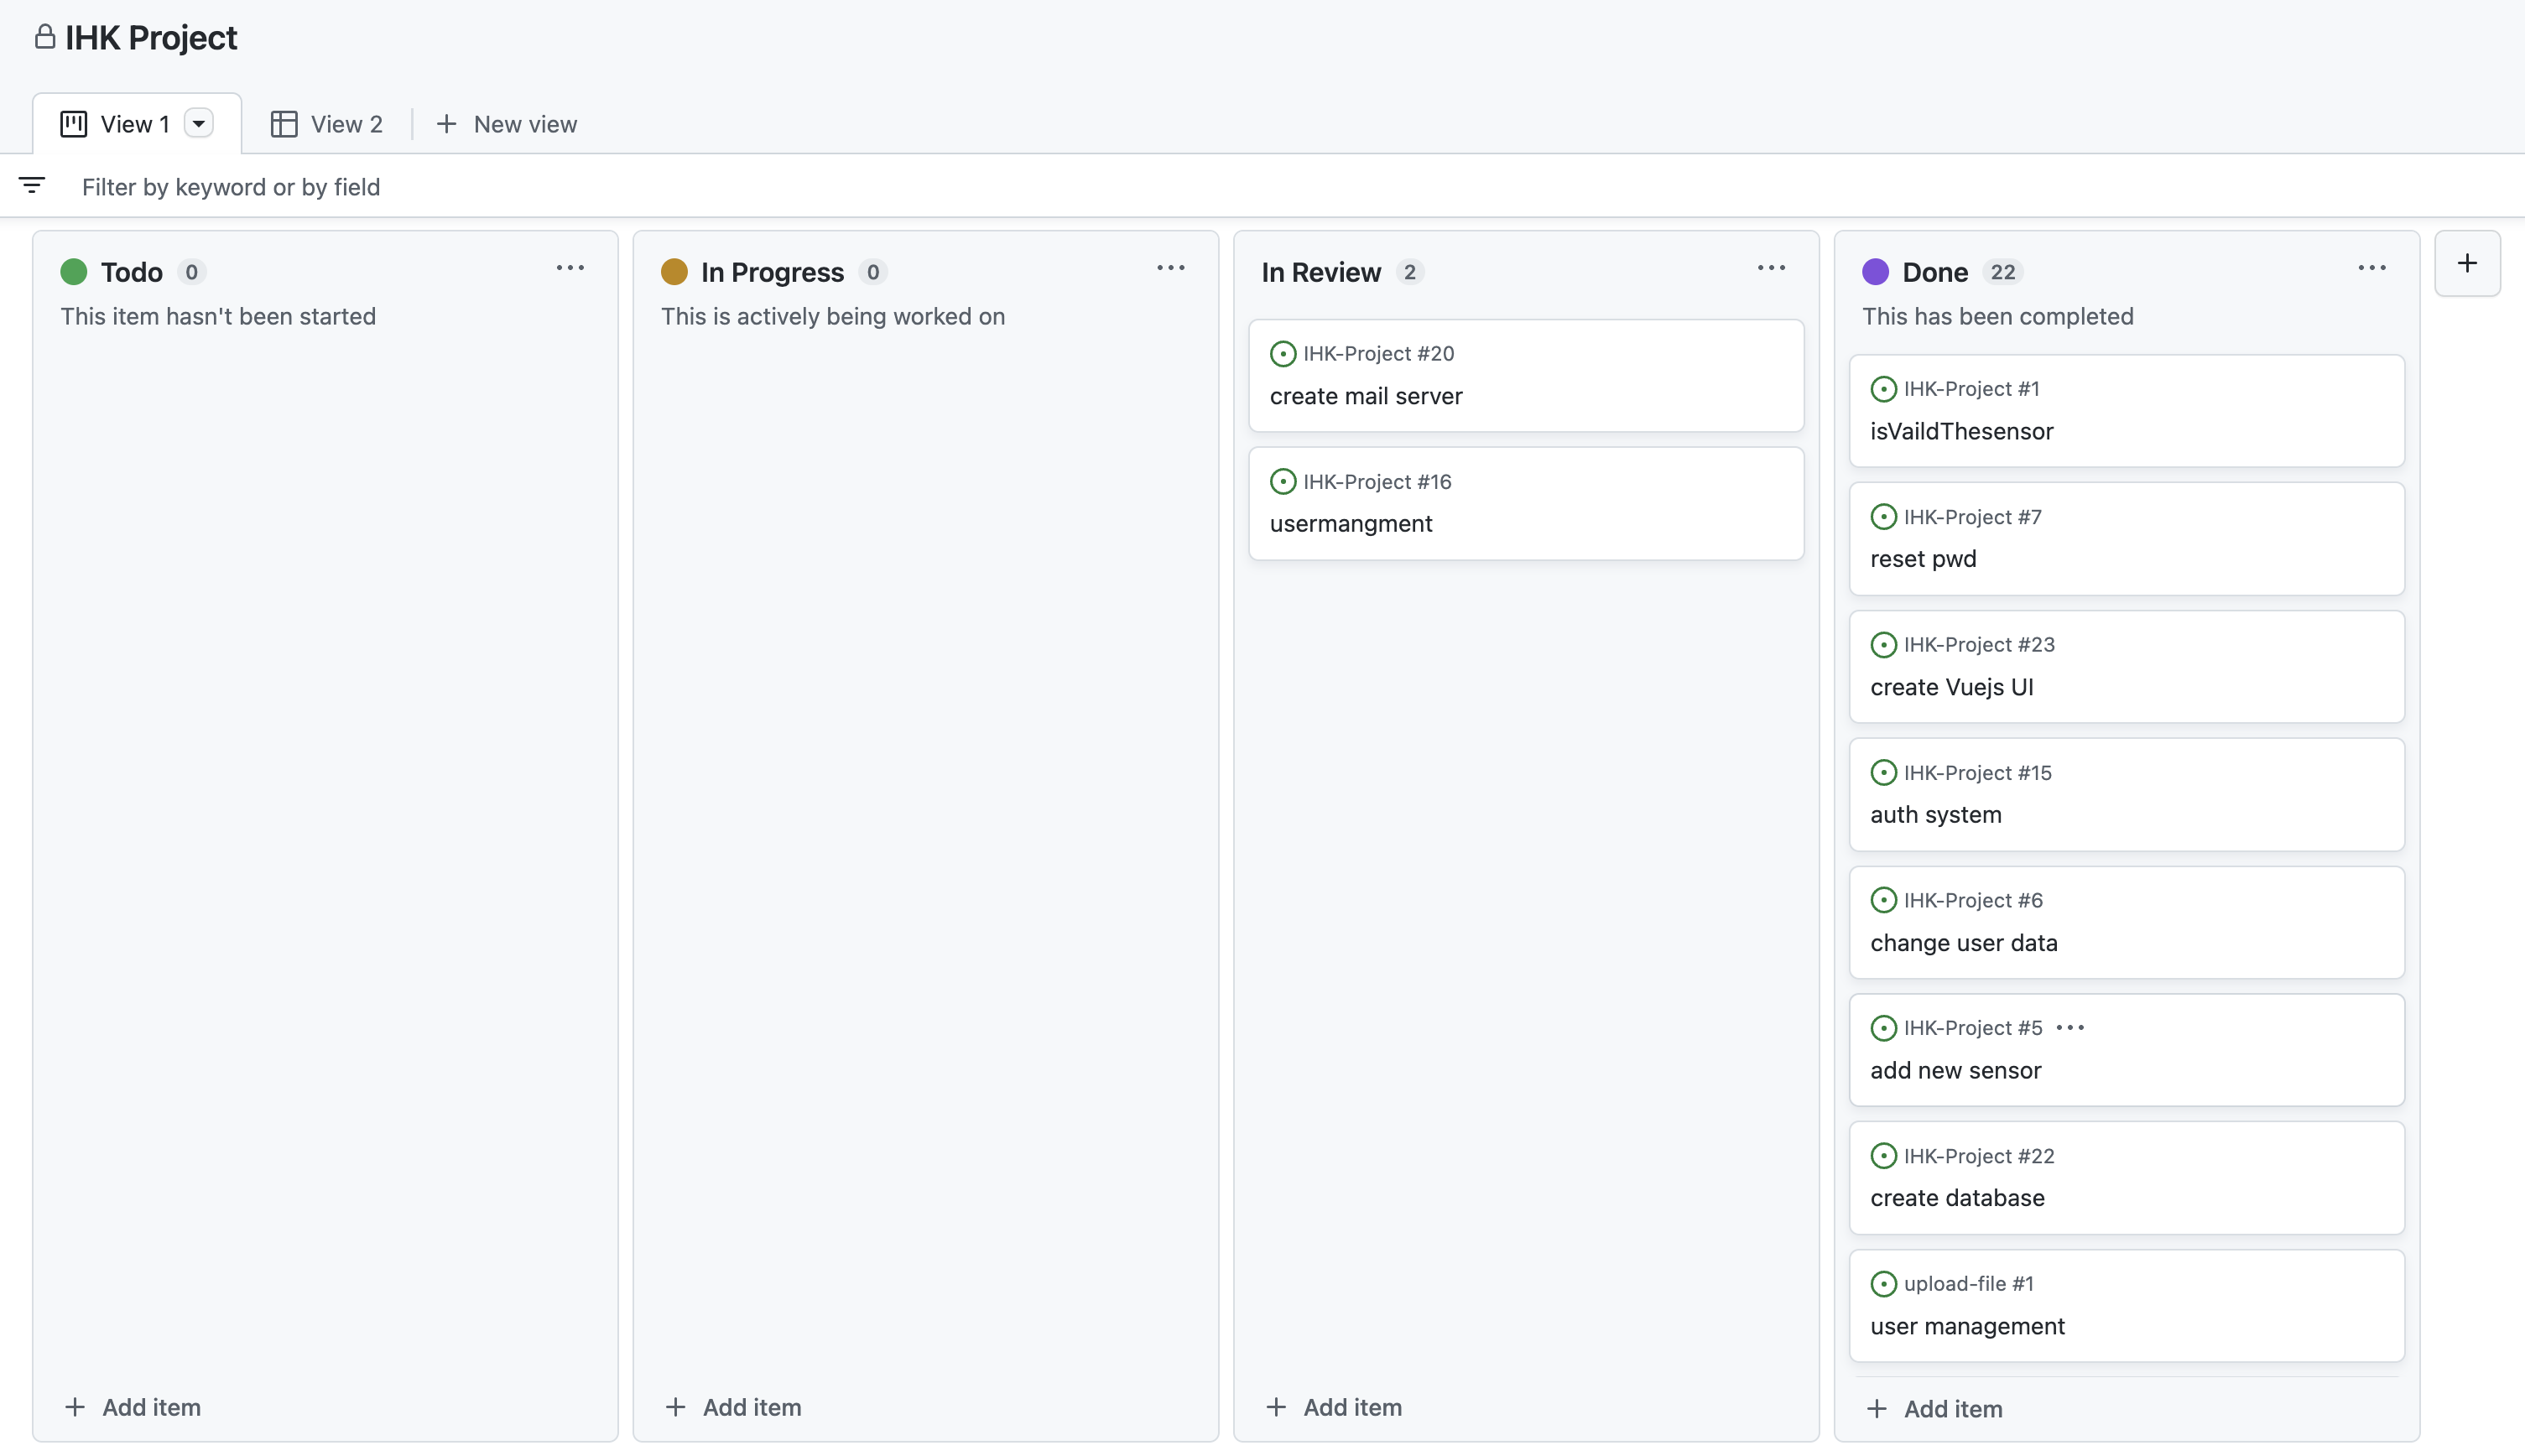
\includegraphics[width=1\textwidth]{img/github_canban.png}
	\caption{Screenshot des Sprint-Boards in GitHub}
	\label{Screenshot des Sprint-Boards in GitHub}
\end{figure}
\clearpage

\subsection{Verwendung von Gantt-Diagramm in GitHub für die Projektplanung}\label{appendix:b2}\par

Seitdem GitHub die Unterstützung für Gantt-Diagramme in seinem Feature-Set integriert hat, ist die Planung und Verfolgung von Projekten einfacher geworden. Durch die Verwendung von Gantt-Diagrammen in GitHub können die verschiedenen Phasen des Projekts, Meilensteine und Aufgaben übersichtlich dargestellt und der Fortschritt sowie die Abhängigkeiten zwischen den einzelnen Aufgaben verfolgt werden. Dies trägt zur effektiven Planung, Zeitmanagement und zur rechtzeitigen Erreichung der Projektziele bei.
\begin{figure}[htbp]
	\centering
	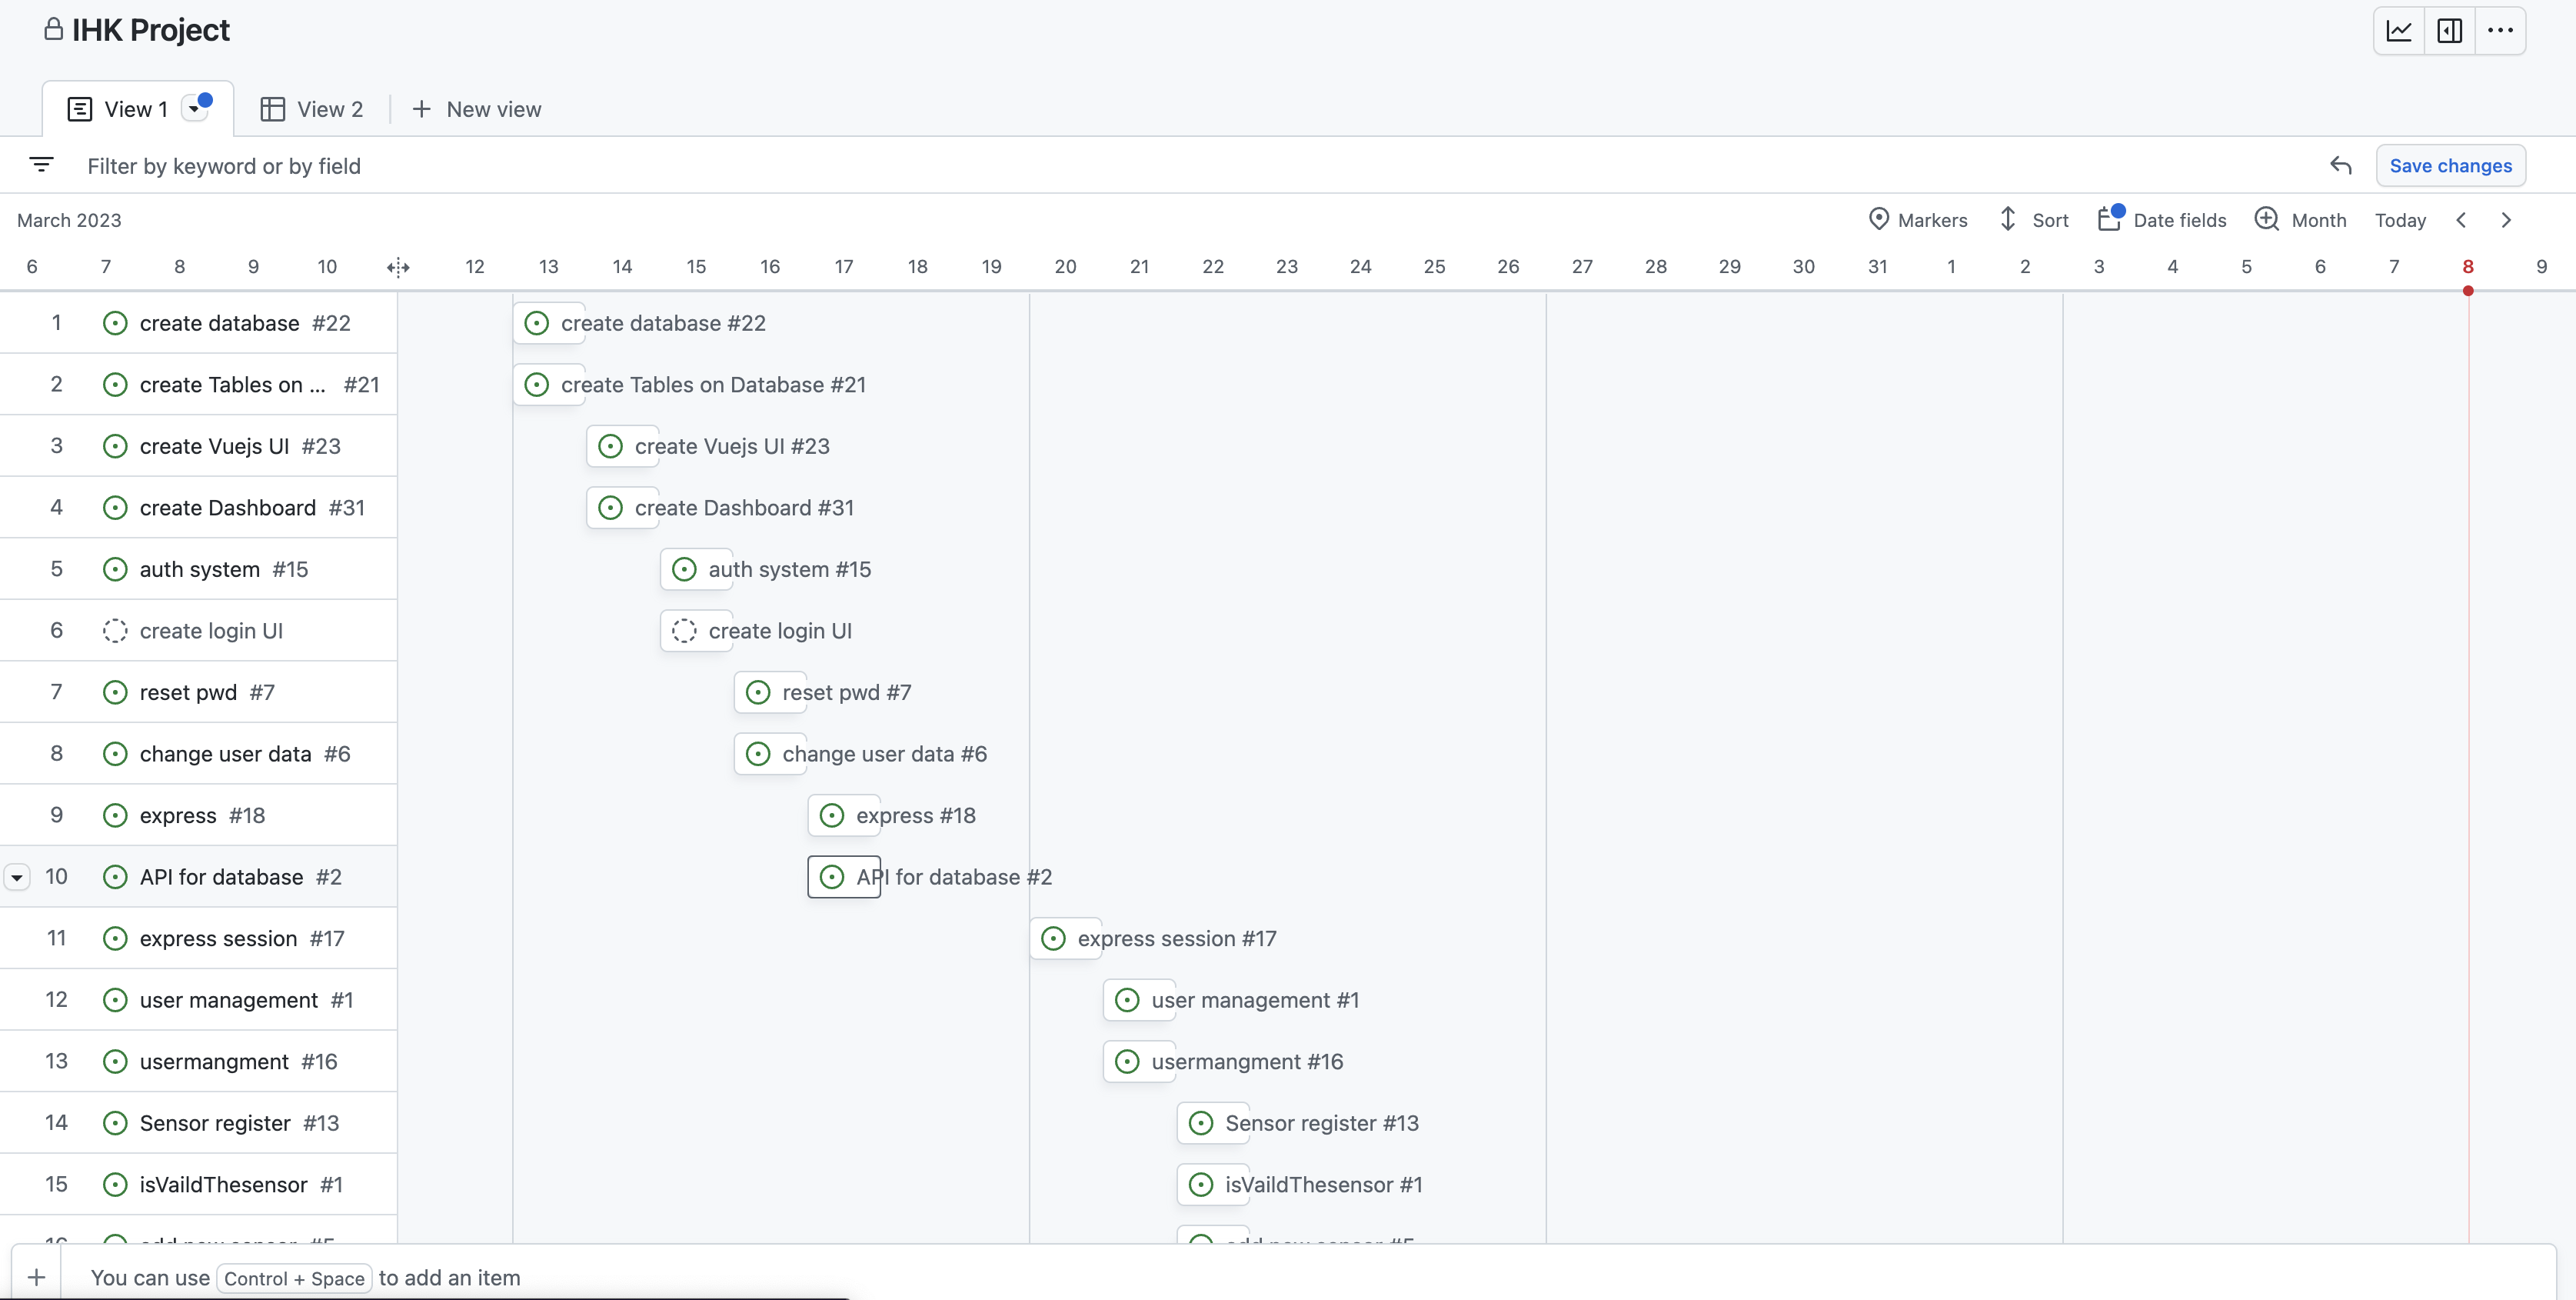
\includegraphics[width=1\textwidth]{img/github_diaramm.png}
	\caption{Verwendung von Gantt-Diagramm in GitHub für die Projektplanung}
	\label{Verwendung von Gantt-Diagramm in GitHub für die Projektplanung}
\end{figure}
\clearpage

\subsection{Screenshot des File-Trees Backend}\label{appendix:b5}\par
Das Projekt wurde mit einer sorgfältig durchdachten Ordnerstruktur als Back-End entwickelt, um eine hohe Organisationsstruktur und Fehlerfreiheit zu gewährleisten.
Durch die präzise Aufteilung der Dateien und Verzeichnisse ist es einfach, Probleme zu finden und zu beheben.
Auf diese Weise können wir eine reibungslose Funktionsweise unseres Produkts sicherstellen und die Benutzererfahrung optimieren.
\begin{figure}[htbp]
	\centering
	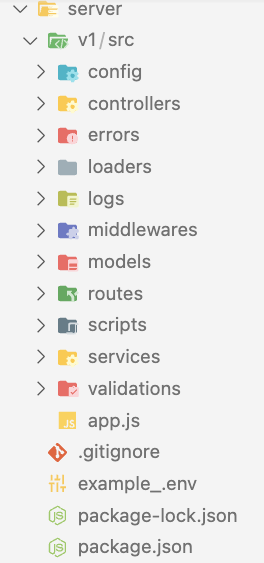
\includegraphics[width=100px]{img/vsd.png}
	\caption{Screenshot des File-Trees Backend}
\end{figure}
\clearpage


\subsection{Anmeldung eines neuen Sensors}\label{appendix:b3}\par
Im folgenden Abschnitt wird ein \acs{JSON} beschrieben, das einen Sensor mit dem Datentyp “integer” repräsentiert.


Mit diesem \acs{JSON} kann der Sensor seine Daten und Einstellungen an das Backend senden, um beispielsweise Daten an das Frontend zu senden oder die Daten in der Datenbank zu speichern. Das Backend verwendet diese Informationen, um den Sensor zu verwalten und seine Konfiguration zu aktualisieren.
	\begin{lstlisting}[caption={Anmeldung eines neuen Sensors (Backend)  JSON-Modell}, style=js]
		{
			sensor_name: 'Anrufe pro Stunde',
			sensor_type: 'process',
			data_type: 'integer',
			unit: 'anrufe',
			unit_display: 'Anrufe/h',
			refresh_interval: 60,
			data_source: 'htts://192.168.12.31:4000',
			data_parser: '',
			sensor_max: 1000,
			sensor_min: 0,
			show: true,
			saveData: true,
			DataRetentionPeriodInMonths: 6,
			visible: true,
			Data: ''
		}
	\end{lstlisting}
\clearpage



	\begin{lstlisting}[caption={Anmeldung eines neuen Sensors (Backend)}, style=js]
		// Function to validate if all required fields are present in the sensor data object
		const validateSensorData = (sensorData) => {
			// List of all required fields
			const requiredFields = [
				"sensor_name",
				"sensor_type",
				"data_type",
				"unit",
				"unit_display",
				"refresh_interval",
				"data_source",
				"data_parser",
				"sensor_max",
				"sensor_min",
				"visible",
				"Data",
				"show",
				"saveData",
				"DataRetentionPeriodInMonths",
			];

			// Check if each required field exists in the sensor data object
			// If any required field is missing, return false
			requiredFields.forEach((field) => {
				if (!sensorData.hasOwnProperty(field)) {
					return false;
				}
			});

			// If all required fields are present, return true
			return true;
		};

		// Route to register a new sensor
		app.post('/registerSensor', async (req, res) => {
			const sensorData = req.body;

			// Validate if all required fields are present in the sensor data object
			if (!validateSensorData(sensorData)) {
				// If any required field is missing, return an error response
				res.status(400).json({
					code: 113,
					message: 'Fehlende oder ungueltige Sensorinformationen',
				});
				return;
			}

			// Add the sensor to the database
			try {
				// Establish a database connection
				const connection = await db.getConnection();

				// SQL query to insert the sensor data into the database
				const sql = `
				INSERT INTO sensors (sensor_name, sensor_type, data_type, unit, unit_display, refresh_interval, data_source, sensor_max, sensor_min, visible, data, show, saveData, DataRetentionPeriodInMonths)
				VALUES (?, ?, ?, ?, ?, ?, ?, ?, ?, ?, ?, ?, ?, ?, ?);
			 `;

				// Parameters for the SQL query
				const params = [
					sensorData.sensor_name,
					sensorData.sensor_type,
					sensorData.data_type,
					sensorData.unit,
					sensorData.unit_display,
					sensorData.refresh_interval,
					sensorData.data_source,
					sensorData.data_parser,
					sensorData.sensor_max,
					sensorData.sensor_min,
					sensorData.visible,
					sensorData.Data || '',
					sensorData.show,
					sensorData.saveData,
					sensorData.DataRetentionPeriodInMonths,
				];

				// Execute the SQL query
				const result = await connection.query(sql, params);

				// Get the sensor ID of the newly inserted sensor
				const sensorId = result.insertId;

				// Close the database connection
				await connection.end();

				// Send a success response with the sensor ID
				res.status(201).json({
					message: 'Sensor erfolgreich registriert',
					code: 207,
					sensor_id: sensorId,
				});
			} catch (error) {
				// If there is an error while adding the sensor, return an error response
				console.error('Error adding sensor:', error);
				res.status(500).json({
					message: 'Fehler beim Registrieren des Sensors',
					code: 212,
				});
			}
		});
	\end{lstlisting}
\clearpage


	\begin{lstlisting}[caption={Anmeldung eines neuen Sensors (Backend) Unit-Tests}, style=js]
		describe('Sensor API Tests', () => {
			it('should register a new sensor', async () => {
				const sensorData = {
					sensor_name: 'Anrufe pro Stunde',
					sensor_type: 'process',
					data_type: 'integer',
					unit: 'anrufe',
					unit_display: 'Anrufe/h',
					refresh_interval: 60,
					data_source: 'htts://192.168.12.31:4000',
					data_parser: '',
					sensor_max: 1000,
					sensor_min: 0,
					show: true,
					DataRetentionPeriodInMonths: 6,
					visible: true,
					Data: ''
				};
				const res = await request(app).post('/registerSensor').send(sensorData);
				expect(res.statusCode).toEqual(201);
				expect(res.body.message).toEqual('Sensor erfolgreich registriert');
				expect(res.body.sensor_id).toBeDefined();
			});

			it('should return an error message if sensor data is incomplete', async () => {
				const sensorData = {
					sensor_name: 'Anrufe pro Stunde',
					sensor_type: 'process',
					data_type: 'integer',
					unit: 'anrufe',
					unit_display: 'Anrufe/h',
					refresh_interval: 60,
					data_source: 'htts://192.168.12.31:4000',
					data_parser: '',
					sensor_max: 1000,
					sensor_min: 0,
					show: true
				};
				const res = await request(app).post('/registerSensor').send(sensorData);
				expect(res.statusCode).toEqual(400);
				expect(res.body.message).toEqual('Fehlende oder ungueltige Sensorinformationen');
			});
		});
	\end{lstlisting}
\clearpage


\begin{figure}[htbp]
	\centering
	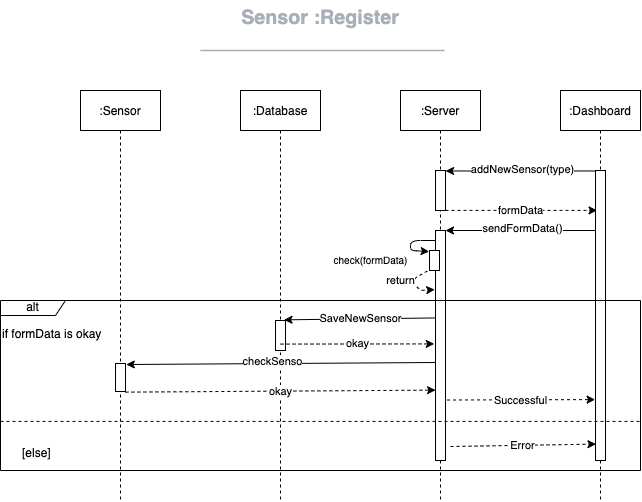
\includegraphics[width=1\textwidth]{img/register_sequence_Diagramm.png}
	\caption{Anmeldung eines neuen Sensors Sequenzdiagramm}
\end{figure}
\clearpage

\subsection{Sequenzdiagramm: Sensor schickt Daten}\label{appendix:b4}\par

In diesem Sequenzdiagramm wird dargestellt, wie der Sensor Daten an den Server sendet und wie der Server die Daten in der Datenbank speichert. Außerdem wird gezeigt, wie das Dashboard die Daten aktualisiert:
\begin{itemize}
	\item Der Sensor erfasst Daten und sendet sie an den Server.
	\item Der Server empfängt die Daten und verarbeitet sie.
	\item Der Server speichert die verarbeiteten Daten in der Datenbank.
	\item Das Dashboard fordert regelmäßig aktualisierte Daten von der Datenbank an.
	\item Der server sendet die angeforderten Daten an das Dashboard.
	\item Das Dashboard aktualisiert die angezeigten Daten entsprechend den neuen Daten.
\end{itemize}

Durch diese Darstellung wird der Datenfluss von der Erfassung durch den Sensor bis zur Anzeige auf dem Dashboard verdeutlicht.

\begin{figure}[h]
	\centering
	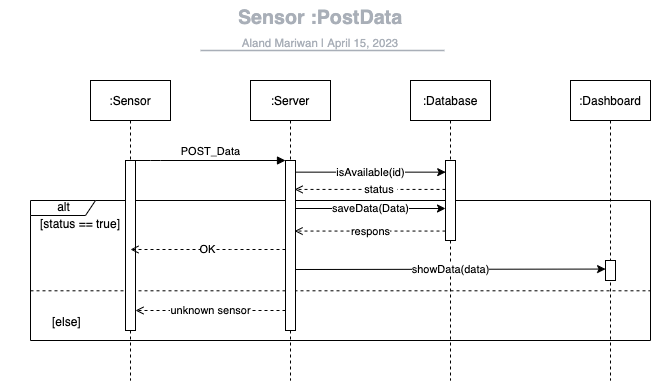
\includegraphics[width=1\textwidth]{img/postData_sequence_Diagramm.png}
	\caption{Sensor schickt Daten (Sequenzdiagramm)}
\end{figure}
\clearpage




\begin{lstlisting}[caption={Sensor schickt Daten (Backend)}, style=js]
	router.get('sensor/:id/data', async (req, res) => {
		try {
			const sensorId = req.params.id;
			const sensor = await db.getSensorById(sensorId);
			if (!sensor) {
				res.status(404).json({
					message: 'Sensor nicht gefunden',
					code: 112,
				});
				return;
			}
			const data = await db.getLastestSensorData(sensorId);
			if (!data) {
				res.status(204).json({
					message: 'Keine Daten vorhanden',
					code: 113,
				});
				return;
			}
			res.status(200).json({
				data: data,
				message: 'Daten gesendet',
				code: 201,
			});
		} catch (err) {
			console.error(err);
			res.status(500).json({ message: 'DB Error', code: 401 });
		}
	});
\end{lstlisting}

	\begin{lstlisting}[caption={Sensor schickt Daten (Backend) Unit-Tests }, style=js]

		describe('GET /sensor/:id/data', () => {
			beforeEach(() => {
			  jest.spyOn(db, 'getSensorById').mockImplementation(async (id) => {
				 if (id === '123') {
					return { id: '123', name: 'Test Sensor' };
				 }
				 return null;
			  });

			  jest.spyOn(db, 'getLastestSensorData').mockImplementation(async (id) => {
				 if (id === '123') {
					return { id: '456', sensorId: '123', value: 10 };
				 }
				 return null;
			  });
			});

			afterEach(() => {
			  jest.restoreAllMocks();
			});

			it('should return 404 if sensor not found', async () => {
			  const res = await request(app).get('/sensor/456/data');

			  expect(res.status).toBe(404);
			  expect(res.body.message).toBe('Sensor nicht gefunden');
			  expect(res.body.code).toBe(112);
			});

			it('should return 204 if no data available', async () => {
			  const res = await request(app).get('/sensor/123/data');

			  expect(res.status).toBe(204);
			  expect(res.body.message).toBe('Keine Daten vorhanden');
			  expect(res.body.code).toBe(113);
			});

			it('should return latest data for the sensor', async () => {
			  const res = await request(app).get('/sensor/123/data');

			  expect(res.status).toBe(200);
			  expect(res.body.message).toBe('Daten gesendet');
			  expect(res.body.code).toBe(201);
			  expect(res.body.data.id).toBe('456');
			  expect(res.body.data.sensorId).toBe('123');
			  expect(res.body.data.value).toBe(10);
			});

			it('should handle database errors', async () => {
			  jest.spyOn(db, 'getSensorById').mockImplementation(async () => {
				 throw new Error('Database error');
			  });

			  const res = await request(app).get('/sensor/123/data');

			  expect(res.status).toBe(500);
			  expect(res.body.message).toBe('DB Error');
			  expect(res.body.code).toBe(401);
			});
		 });
	\end{lstlisting}
\clearpage




	\begin{lstlisting}[caption={Neue Benutzer hinzufügen (Backend)}, style=js]
		router.post('/register', function (req, res) {
			let name = decrypt(req.body.name);
			let lastname = decrypt(req.body.lastname);
			let username = decrypt(req.body.username);
			let email = decrypt(req.body.email);
			let password = decrypt(req.body.password);

			if (
				name === false ||
				lastname === false ||
				username === false ||
				email === false ||
				password === false
			) {
				res.status(400).send({
					msg: 'Anfrage nicht gueltig',
					code: 101,
				});
				return;
			}
			username = username.toLowerCase();
			email = email.toLowerCase();

			if (!isEmail(email)) {
				res.status(400).send({
					msg: 'E-Mail existiert nicht',
					code: 105,
				});
				return;
			}

			if (!checkUsername(username)) {
				res.status(400).send({
					msg: 'Benutzername hat ungueltige Zeichen',
					code: 107,
				});
				return;
			}

			if (password.length < 8) {
				res.status(400).send({
					msg: 'Kennwort Mindestlaenge ist 8 Zeichen',
					code: 106,
				});
				return;
			}

			db.query(
				'SELECT * FROM users WHERE username = ? OR email = ?',
				[username, email],
				function (err, result) {
					if (err) {
						console.error(err);
						res.status(500).send({
							msg: 'DB Error',
							code: 401,
							err: err,
						});
						return;
					}

					if (result.length != 0) {
						res.status(500).send({
							msg: 'Benutzername oder E-Mail bereits registriert',
							code: 104,
						});
						return;
					}

					bcrypt.hash(password, saltRounds, function (err2, hash) {
						if (err2) {
							console.error(err2);
							res.status(500).send({
								msg: 'Bycrypt Error',
								code: 402,
								err: err2,
							});
							return;
						}

						db.query(
							'INSERT INTO users (name, lastname, username, email, password ) VALUE (?,?,?,?,?)',
							[name, lastname, username, email, hash],
							function (error, response) {
								if (error) {
									console.error(error);
									res.status(500).send({
										msg: 'DB Error',
										code: 401,
										err: error,
									});
									return;
								}

								res.status(200).send({
									msg: 'Benutzer registriert',
									code: 202,
								});
							},
						);
					});
				},
			);
		});
	\end{lstlisting}
\clearpage

	\begin{lstlisting}[caption={Neue Benutzer hinzufügen (Backend) Unit-Tests}, style=js]
		describe('POST /auth/register', () => {
			test('should return 400 if request is invalid', async () => {
				var nameHash = encrypt('invalid');
				var lastnameHash = encrypt('request');
				var usernameHash = encrypt('invalid');
				var emailHash = encrypt('invalid');
				var passwordHash = bcrypt.hashSync('short', saltRounds); // hash created
				const response = await request(app)
					.post('/auth/register')
					.send({
						name: nameHash,
						lastname: lastnameHash,
						username: usernameHash,
						email: emailHash,
						password: passwordHash,
					})
					.set('Content-Type', 'application/json');

				expect(response.status).toBe(400);
				expect(response.body.msg).toBe('Anfrage nicht gueltig');
				expect(response.body.code).toBe(101);
			});

			test('should return 400 if email is invalid', async () => {
				var nameHash = encrypt('Aland');
				var lastnameHash = encrypt('Mariwan');
				var usernameHash = encrypt('amariwan');
				var emailHash = encrypt('invalid');
				var passwordHash = bcrypt.hashSync('short1234568', saltRounds); // hash created
				const response = await request(app)
					.post('/auth/register')
					.send({
						name: nameHash,
						lastname: lastnameHash,
						username: usernameHash,
						email: emailHash,
						password: passwordHash,
					})
					.set('Content-Type', 'application/json');

				expect(response.status).toBe(400);
				expect(response.body.msg).toBe('E-Mail existiert nicht');
				expect(response.body.code).toBe(105);
			});

			test('should return 400 if username has invalid characters', async () => {
				var nameHash = encrypt('Aland');
				var lastnameHash = encrypt('Mariwan');
				var usernameHash = encrypt('amariwan.99');
				var emailHash = encrypt('dev@aland-mariwan.de');
				var passwordHash = bcrypt.hashSync('short1234568', saltRounds); // hash created
				const response = await request(app)
					.post('/auth/register')
					.send({
						name: nameHash,
						lastname: lastnameHash,
						username: usernameHash,
						email: emailHash,
						password: passwordHash,
					})
					.set('Content-Type', 'application/json');

				expect(response.status).toBe(400);
				expect(response.body.msg).toBe('Benutzername hat ungueltige Zeichen');
				expect(response.body.code).toBe(107);
			});

			test('should return 400 if password is too short', async () => {
				var nameHash = encrypt('Aland');
				var lastnameHash = encrypt('Mariwan');
				var usernameHash = encrypt('amariwan.99');
				var emailHash = encrypt('dev@aland-mariwan.de');
				var passwordHash = bcrypt.hashSync('short', saltRounds); // hash created
				const response = await request(app)
					.post('/auth/register')
					.send({
						name: nameHash,
						lastname: lastnameHash,
						username: usernameHash,
						email: emailHash,
						password: passwordHash,
					})
					.set('Content-Type', 'application/json');

				expect(response.status).toBe(400);
				expect(response.body.msg).toBe('Kennwort Mindestlaenge ist 8 Zeichen');
				expect(response.body.code).toBe(106);
			});
		});
	\end{lstlisting}
\clearpage




\begin{lstlisting}[caption={Passwort zurücksetzen (Backend)}, style=js]
	// Generate a token and send it to the user's email
	const token = crypto.randomBytes(1000).toString('hex');
	const transporter = nodemailer.createTransport(config.mailAuth[0]);
	const html = fs.readFileSync('htmlMail/forgotPassword.html').toString();
	const mailOptions = {
		from: {
			name: 'GMS Passwort vergessen',
			address: config.mailAuth[0].auth.user,
		},
		to: email,
		subject: 'GMS Passwort Aenderung',
		html: html
			.replace('${__NAME__}', user.data.lastname)
			.replace('${__HOST__}', config.frontend_host)
			.replace('${__TOKEN__}', token),
	};
	transporter.sendMail(mailOptions, async (err, info) => {
		if (err) {
			console.error(err);
			res.status(400).send({
				msg: `Mail Error`,
				code: 403,
				err: err,
			});
			return;
		}
		const isSetUserTokenOnDB = await setUserTokenOnDB(token, email);
		if (isSetUserTokenOnDB.result === 0) {
			res.status(400).send({
				msg: 'Benutzer nicht gefunden',
				code: 110,
			});
			return;
		}
		if (isSetUserTokenOnDB.result === 1) {
			//DB Error
			console.error(user.err);
			res.status(500).send({
				msg: 'DB Error',
				code: 401,
				err: user.err,
			});
			return;
		}
		res.status(200).send({
			msg: `E-Mail gesendet`,
			code: 211,
		});
	});
});
\end{lstlisting}
\clearpage


\subsection{Dashboard-Seite}\label{appendix:b5}\par
\begin{figure}[htbp]
	\centering
	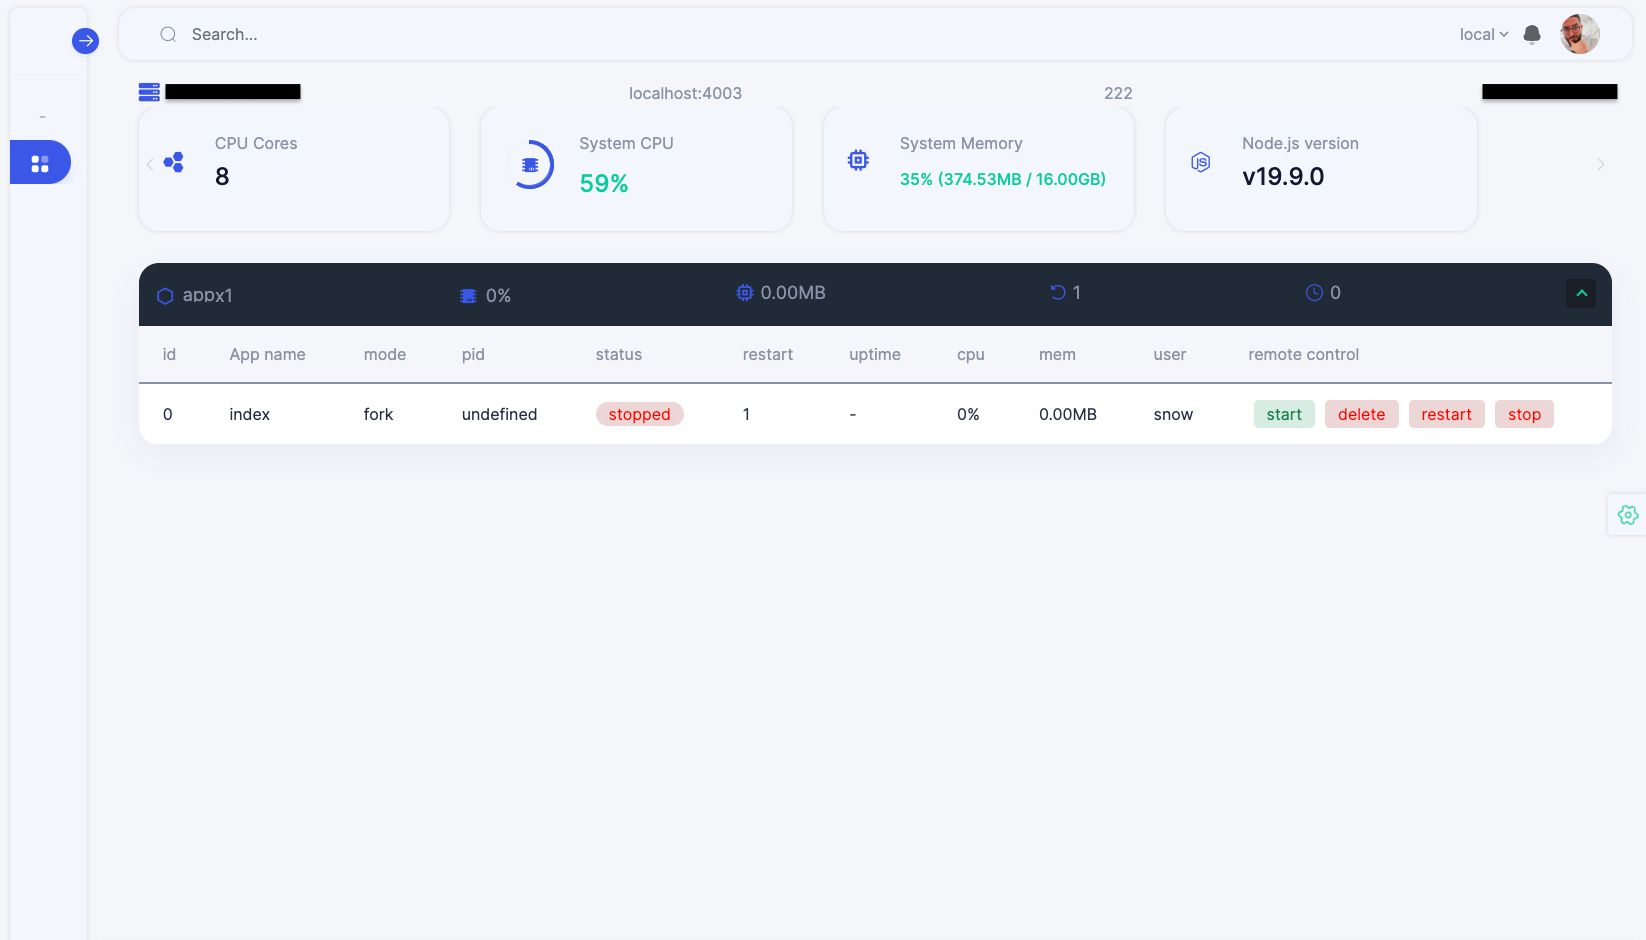
\includegraphics[width=1\textwidth]{img/dashboard.png}
	\caption{Dashboard-Seite (Frontend)}
\end{figure}
\clearpage

	\begin{lstlisting}[caption={VueJs router (Frontend)}, style=js]
		// Dashboard routes
		const dashboardRoutes = (prefix) => [
		  {
			 path: '',
			 name: prefix + '.dashboard',
			 meta: { auth: true, name: 'Home', isBanner: false },
			 component: () => import('@/views/dashboards/IndexPage.vue')
		  }
		]
		// Default routes
		const defaultChildRoutes = (prefix) => [
		  {
			 path: '',
			 name: prefix + '.dashboard',
			 meta: { auth: true, name: 'Home', isBanner: false },
			 component: () => import('@/views/dashboards/IndexPage.vue')
		  },
		  // Spacial Pages
		  {
			 path: '/server',
			 name: prefix + '.server',
			 meta: { auth: true, name: 'Server', isBanner: false },
			 component: () => import('@/views/spacial-pages/serverPage.vue')
		  },
		  {
			 path: '/sensor',
			 name: prefix + '.sensor',
			 meta: { auth: true, name: 'Sensor', isBanner: false },
			 component: () => import('@/views/spacial-pages/sensorPage.vue')
		  },
		  {
			 path: '/setting',
			 name: prefix + '.setting',
			 meta: { auth: true, name: 'Setting', isBanner: false },
			 component: () => import('@/views/spacial-pages/settingPage.vue')
		  },
		  // Users Pages
		  {
			 path: '/sensor-list',
			 name: prefix + '.sensor-list',
			 meta: { auth: true, name: 'Sensor List', isBanner: false },
			 component: () => import('@/views/sensor/ListPage.vue')
		  },
		  {
			 path: '/sensor-add',
			 name: prefix + '.sensor-add',
			 meta: { auth: true, name: 'Sensor Add', isBanner: false },
			 component: () => import('@/views/sensor/AddPage.vue')
		  },
		  {
			 path: '/user-profile',
			 name: prefix + '.user-profile',
			 meta: { auth: true, name: 'User Add', isBanner: false },
			 component: () => import('@/views/user/ProfilePage.vue')
		  },
		  {
			 path: '/charts',
			 name: prefix + '.charts',
			 meta: { auth: true, name: 'Charts', isBanner: false },
			 component: () => import('@/views/charts/charts.vue')
		  },
		  {
			 path: '/validation',
			 name: prefix + '.validation',
			 meta: { auth: true, name: 'Validation', isBanner: false },
			 component: () => import('@/views/forms/ValidationPage.vue')
		  },
		  // Table Pages
		  {
			 path: '/table',
			 name: prefix + '.table',
			 meta: { auth: true, name: 'Table', isBanner: false },
			 component: () => import('@/views/tables/Table.vue')
		  },
		  // Admin Pages
		  {
			 path: '/admin-permissions',
			 name: prefix + '.admin-permissions',
			 meta: { auth: true, name: 'Admin Permissions', isBanner: false },
			 component: () => import('@/views/admin/AdminPage.vue')
		  }
		]

		const errorRoutes = (prefix) => [
		  // Error Pages
		  {
			 path: '404',
			 name: prefix + '.404',
			 meta: { auth: true, name: 'Error 404', isBanner: false },
			 component: () => import('@/views/errors/Error404Page.vue')
		  },
		  {
			 path: '500',
			 name: prefix + '.500',
			 meta: { auth: true, name: 'Error 500', isBanner: false },
			 component: () => import('@/views/errors/Error500Page.vue')
		  },
		  {
			 path: 'maintenance',
			 name: prefix + '.maintenance',
			 meta: { auth: true, name: 'Maintenance', isBanner: false },
			 component: () => import('@/views/errors/MaintenancePage.vue')
		  }
		]
	\end{lstlisting}

\clearpage


	\begin{lstlisting}[caption={registerSensor (Frontend)}, style=js]
		<template>
			<div class="register-sensor">
				<h2>Neuen Sensor registrieren</h2>
				<form @submit.prevent="registerSensor">
					<label for="sensor_name">Sensor Name:</label>
					<input type="text" id="sensor_name" v-model="sensorData.sensor_name" required>
					<label for="sensor_type">Sensor Typ:</label>
					<input type="text" id="sensor_type" v-model="sensorData.sensor_type" required>
					<label for="data_type">Datentyp:</label>
					<input type="text" id="data_type" v-model="sensorData.data_type" required>
					<label for="unit">Einheit:</label>
					<input type="text" id="unit" v-model="sensorData.unit" required>
					<label for="unit_display">Einheitsanzeige:</label>
					<input type="text" id="unit_display" v-model="sensorData.unit_display" required>
					<label for="refresh_interval">Aktualisierungsintervall:</label>
					<input type="text" id="refresh_interval" v-model="sensorData.refresh_interval" required>
					<label for="data_source">Datenquelle:</label>
					<input type="text" id="data_source" v-model="sensorData.data_source" required>
					<label for="data_parser">Daten-Parser:</label>
					<input type="text" id="data_parser" v-model="sensorData.data_parser" required>
					<label for="sensor_max">Maximalwert:</label>
					<input type="text" id="sensor_max" v-model="sensorData.sensor_max" required>
					<label for="sensor_min">Minimalwert:</label>
					<input type="text" id="sensor_min" v-model="sensorData.sensor_min" required>
					<label for="visible">Sichtbarkeit:</label>
					<input type="checkbox" id="visible" v-model="sensorData.visible">
					<label for="data">Daten:</label>
					<textarea id="data" v-model="sensorData.Data"></textarea>
					<label for="show">Anzeigen:</label>
					<input type="checkbox" id="show" v-model="sensorData.show">
					<label for="saveData">Daten speichern:</label>
					<input type="checkbox" id="saveData" v-model="sensorData.saveData">
					<label for="DataRetentionPeriodInMonths">Datenspeicherzeit:</label>
					<input type="text" id="DataRetentionPeriodInMonths" v-model="sensorData.DataRetentionPeriodInMonths" required>
					<button type="submit">Sensor registrieren</button>
				</form>
				<div v-if="errorMessage" class="error-message">{{ errorMessage }}</div>
				<div v-if="successMessage" class="success-message">{{ successMessage }}</div>
			</div>
		</template>

		<script>
		export default {
		  data() {
			 return {
				// Hier kommen die Formularfelder als data-Properties hin
				sensor_name: "",
				sensor_type: "",
				data_type: "",
				unit: "",
				unit_display: "",
				refresh_interval: "",
				data_source: "",
				data_parser: "",
				sensor_max: "",
				sensor_min: "",
				visible: "",
				Data: "",
				show: "",
				saveData: "",
				DataRetentionPeriodInMonths: "",
			 };
		  },
		  methods: {
			 async registerSensor() {
				// Erstelle das Sensorobjekt mit den Formulardaten
				const sensorData = {
				  sensor_name: this.sensor_name,
				  sensor_type: this.sensor_type,
				  data_type: this.data_type,
				  unit: this.unit,
				  unit_display: this.unit_display,
				  refresh_interval: this.refresh_interval,
				  data_source: this.data_source,
				  data_parser: this.data_parser,
				  sensor_max: this.sensor_max,
				  sensor_min: this.sensor_min,
				  visible: this.visible,
				  Data: this.Data,
				  show: this.show,
				  saveData: this.saveData,
				  DataRetentionPeriodInMonths: this.DataRetentionPeriodInMonths,
				};

				try {
				  // Sende das Sensorobjekt an den Server
				  const response = await axios.post("/registerSensor", sensorData);

				  // Wenn die Sensorregistrierung erfolgreich war, zeige eine Erfolgsmeldung an
				  if (response.data.code === 207) {
					 alert(`Sensor erfolgreich registriert mit ID ${response.data.sensor_id}`);
				  }
				} catch (error) {
				  // Wenn es einen Fehler gab, zeige eine Fehlermeldung an
				  alert("Fehler beim Registrieren des Sensors");
				  console.error(error);
				}
			 },
		  },
		};
		</script>
	\end{lstlisting}

	\begin{lstlisting}[caption={sort Function (Frontend)}, style=js]
	/* Used to sort the data.
		This function sorts an array of objects by a given property, either in ascending or descending order.
		It also converts any dates in the given property to ISO format before sorting,
		and converts them back to the original format after sorting.
		*/
const sortByProperty = (arr, prop, sortOrder, nullText) =>
{
	log(arr, prop, sortOrder, nullText);
	try {
		if (arr == null || arr.length <= 0) return false;
		if (prop == null || prop.length <= 0) return false;
		if (sortOrder == null || sortOrder.length <= 0) return false;
		const dateRegex = /(\d{1,2})\.(\d{1,2})\.(\d{4}) (\d{1,2}):(\d{1,2}):(\d{1,2})/;
		let isDate = false;
		sortOrder = sortOrder === 'asc' ? true : false;
		let resultsArray = [];
		let y = 0;
		// convert date format in object array to ISO format
		if (arr[y][prop] === nullText) y++;
		if (typeof arr[y][prop] === 'string') {
			// if (isNaN(arr[0][prop])) {
			if (arr[y] && arr[y][prop] && arr[y][prop].match(dateRegex)) {
				arr.forEach((e) => {
					var match = e[prop].match(dateRegex);
					if (match) {
						e[prop] = isoDate(match);
						isDate = true;
					}
				});
			}
			// }
		} else {
			if (isNaN(arr[y][prop].value)) {
				if (arr[y] && arr[y][prop].value && arr[y][prop].value.match(dateRegex)) {
					arr.forEach((e) => {
						var match = e[prop].value.match(dateRegex);
						if (match) {
							e[prop].value = isoDate(match);
							isDate = true;
						}
					});
				}
			}
		}
		// Sortieren des Arrays nach der Eigenschaft und der Sortierreihenfolge.
		//sorts the array of objects by the specified property
		//first checks if the value of the property is a string, if so it transforms it to lowercase
		//if the value is an object, it gets the value property
		//if the value is a number, it sorts it as a number
		//if the value is a string, it checks if it has a currency symbol, if so it parses it to a float and sorts it as a number
		//if the value is a string, it sorts it as a string

		resultsArray = arr.sort((a, b) => {
			var aValue = typeof a[ prop ] === 'string' ? a[ prop ].toLowerCase() : a[ prop ];
			var bValue = typeof b[ prop ] === 'string' ? b[ prop ].toLowerCase() : b[ prop ];
			aValue = typeof aValue === 'object' ? aValue.value : aValue;
			bValue = typeof bValue === 'object' ? bValue.value : bValue;

			if (!isNaN(aValue) && !isNaN(bValue)) {
				return sortOrder ? aValue - bValue : bValue - aValue;
			} else if (typeof aValue === 'string' && typeof bValue === 'string') {
				return sortOrder ? aValue.localeCompare(bValue) : bValue.localeCompare(aValue);
			} else {
				return sortOrder ? aValue.localeCompare(bValue) : bValue.localeCompare(aValue);
			}
		});

		if (isDate) {
			resultsArray.forEach((e) => {
				typeof e[prop] === 'string' ? (e[prop] = convertIsoToGermanDate(e[prop])) : (e[prop].value = convertIsoToGermanDate(e[prop].value));
			});
		}
		return resultsArray;
	} catch (error) {
		console.error(error);
	}
};

// This function converts an isoDate to a german date format
const convertIsoToGermanDate = (isoDate) => {
	try {
		// Create a new Date object from the isoDate
		const date = new Date(isoDate);
		// Extract the date, month, and year from the date object
		const day = date.getDate().toString().padStart(2, '0');
		const month = (date.getMonth() + 1).toString().padStart(2, '0');
		const year = date.getFullYear().toString();
		// Extract the hours, minutes, and seconds from the date object
		const hours = date.getHours().toString().padStart(2, '0');
		const minutes = date.getMinutes().toString().padStart(2, '0');
		const seconds = date.getSeconds().toString().padStart(2, '0');
		// Return the date with the format dd.mm.yyyy hh:mm:ss
		return `${day}.${month}.${year} ${hours}:${minutes}:${seconds}`;
	} catch (error) {
		console.error(error);
	}
};

// This function converts a date from the format DD/MM/YYYY to the format YYYY-MM-DD.
const isoDate = (match) => {
	try {
		const year = match[3];
		const month = match[2];
		const day = match[1];
		const hours = match[4];
		const minutes = match[5];
		const seconds = match[6];
		return `${year}-${month}-${day}T${hours}:${minutes}:${seconds}`;
	} catch (error) {
		console.error(error);
	}
};

const sortArrayBasedOnReference = (arrayA, arrayB) => {
	return arrayB.sort((a, b) => {
		const aIndex = arrayA.indexOf(a.text);
		const bIndex = arrayA.indexOf(b.text);

		if (aIndex === -1) {
			return 1;
		}

		if (bIndex === -1) {
			return -1;
		}

		return aIndex - bIndex;
	});
};

const sortArrayByReferenceArray = (arrayA, referenceArray) => {
	const sortedArrayA = new Array(arrayA.length);

	for (const element of referenceArray) {
		const indexInArrayA = arrayA.indexOf(element.text);

		if (indexInArrayA !== -1) {
			sortedArrayA[element.index] = element.text;
		}
	}

	return sortedArrayA.filter((element) => element !== undefined);
};

const mergeArrayBIntoArrayA = (arrayA, arrayB) => {
	const newArrayA = [];

	for (const element of arrayB) {
		const indexInArrayA = arrayA.indexOf(element.text);
		if (indexInArrayA !== -1) {
			newArrayA.push(element.text);
		}
	}

	for (const element of arrayA) {
		if (!newArrayA.includes(element)) {
			newArrayA.push(element);
		}
	}

	return newArrayA;
};
\end{lstlisting}
\begin{lstlisting}[caption={search Function (Frontend)}, style=js]
const search = (lst, searchLst) => {
	try {
		for (let i = 0; i < searchLst.length; i++) {
			const element = searchLst[i];
			/* Searching in a nested object. */
			lst = filterNode(lst, element.Property, element.Text);
		}
		return lst;
	} catch (error) {
		console.error(error);
	}
};

var canSplit = (str, elements) => {
	try {
		var lst = {
			methor: [],
			str: [],
		};
		for (var i = 0; i < elements.length; i++) {
			if ((str || '').split(elements[i]).length > 1) {
				lst.methor.push(elements[i]);
				lst.str.push(str.split(elements[i]));
			}
		}
		return lst;
	} catch (error) {
		console.error(error);
	}
};

const filterNode = (nodes, parts, searchText) => {
	try {
		if (searchText === 'null') searchText = ' ';
		var lst = [];
		log(parts);
		parts = parts.split('.'); //! you must not have . in the propati
		searchText = searchText.split('&');
		if (typeof nodes == 'undefined' && typeof nodes != 'object') {
			console.error('nodes is not an object');
			return;
		}
		for (let k = 0; k < nodes.length; k++) {
			const e = nodes[k];
			/* Getting the keys of the object. */
			let keys = Object.keys(e);
			var x = 0;
			for (let i = 0; i < keys.length; i++) {
				var key = keys[i];
				if (typeof key == 'object') {
					if (typeof keys[i] == 'object') {
						let sublst = filterNode(e[keys[i]], parts[x], searchText);
						 if (sublst != null) {
						 	sublst.forEach((x) => {
						 		lst.push(x);
						 	});
						 }
					}
				} else {
					if (key == parts[x]) {
						var lNode = typeof e[key] == 'object' ? e[key].value : e[key];
						if (lNode == null) {
							if (searchInSubNode(lNode, searchText, parts, x)) {
								lst.push(e);
							}
						} else {
							if (typeof searchText == 'string') {
								if (searchInNode(lNode, searchText)) {
									lst.push(e);
								}
							} else {
								searchText.forEach((element) => {
									if (searchInNode(lNode, element)) {
										lst.push(e);
									}
								});
							}
						}
					}
				}
			}
		}
		return lst;
	} catch (error) {
		console.error(error);
	}
};

// Search in a subnode
/* Searching in a nested object. */
searchInSubNode = (items, searchText, parts, x) => {
	try {
		if (items != null) {
			++x;
			for (let y = 0; y < items.length; y++) {
				const element = items[y];
				var lNodeText = element[parts[x]];
				if (lNodeText != null && typeof lNodeText == 'string') {
					lNodeText = lNodeText.toLowerCase();
					if (lNodeText.includes(searchText)) {
						return true;
					}
				} else if (typeof lNodeText == 'object') {
					if (searchInSubNode(lNodeText, searchText, parts, x)) {
						return true;
					}
				}
			}
		}
		return false;
	} catch (error) {
		console.error(error);
	}
};

/* This function is used to search in a nested object. */
searchInNode = (item, searchText) => {
	try {
		item = String(item);
		/* Converting the item to lower case. */
		item = item.toLowerCase();
		/* Checking if the searchText is in the item. */
		if (typeof searchText == 'string') {
			if (item.includes(searchText.toLowerCase())) {
				return true;
			}
		}
		return false;
	} catch (error) {
		console.error(error);
	}
};
\end{lstlisting}


\clearpage


\end{document}
